\documentclass[paper=a4,oneside,DIV=8,fontsize=12pt, sectionentrydots=true]{scrartcl}

\usepackage[left=3cm,right=2cm,bottom=2cm,top=2cm,footskip=1.4cm,headsep=0.6cm]{geometry}
%\usepackage[ngerman]{babel}
\usepackage[utf8]{inputenc}
\usepackage[T1]{fontenc}
\usepackage{amsmath}
\usepackage{amsthm,amssymb}
\usepackage{graphicx}
\usepackage[hidelinks]{hyperref}
\usepackage{tikz}
\usepackage{colortbl}
\usepackage{multirow}
\usetikzlibrary{arrows.meta,
                chains,
                positioning,
                shapes.geometric
                }
%\usepackage{fancyhdr}
\usepackage{stmaryrd}
\usepackage{enumerate}
\usepackage{setspace}
\usepackage{multirow,array}
\usepackage{caption}
\usepackage{bbm}
\usepackage{amsfonts}
\usepackage{mathtools}
\usepackage{longtable}
\usepackage{blindtext}
\usepackage{tocloft}
\usepackage{booktabs}
\allowdisplaybreaks

\captionsetup[figure]{font=small,labelfont=small}
%\KOMAoption{footnotes}{multiple}
\setstretch{1.5}

\setlength{\parindent}{0pt}

% Bibliography
\usepackage[
    backend=biber,
%    style=numeric-comp,
    style=authoryear,
    sorting=nyt,
    maxbibnames = 99
  ]{biblatex}
\addbibresource{bibliography_thesis.bib} %Imports bibliography file


\newtheoremstyle{dotless}{}{}{\itshape}{}{\bfseries}{}{ }{}

\theoremstyle{dotless}
\newtheorem{question}{Question}
\newtheorem{theorem}{Theorem}[section]
\newtheorem{corollary}{Corollary}[theorem]
\newtheorem{lemma}[theorem]{Lemma}
\newtheorem*{remark}{Remark}
\newtheorem{definition}{Definition}
\newtheorem*{claim}{Claim}
\DeclareMathOperator*{\E}{\text{E}}
\DeclareMathOperator{\EX}{\mathbb{E}}% expected value
\DeclareMathOperator*{\cov}{\text{Cov}}
\DeclareMathOperator*{\var}{\text{Var}}
\DeclareMathOperator*{\Xbold}{\boldsymbol{X}}
\DeclareMathOperator*{\Xbolddot}{\boldsymbol{\Dot{X}}}
\DeclareMathOperator*{\sumi}{\sum_{i=1}^N}
\DeclareMathOperator*{\sumj}{\sum_{j=1}^N}
\DeclareMathOperator*{\sums}{\sum_{s=1}^T}
\DeclareMathOperator*{\sumt}{\sum_{t=1}^T}
\DeclareMathOperator*{\sumtstar}{\sum_{t^* = 1}^T}
\DeclareMathOperator*{\argmax}{arg\,max}
\DeclareMathOperator*{\argmin}{arg\,min}
\DeclareMathOperator*{\A}{\mathbbm{A}}
\DeclareMathOperator*{\indep}{\perp \!\!\! \perp}
\DeclareMathOperator*{\Prob}{\mathbbm{P}}
\DeclareMathOperator*{\plim}{plim}
\DeclareMathOperator*{\indicator}{\textbf{1}}


% Align Roman page numbers
\cftsetpnumwidth{2em}

% Add dots after heading in TOC
\renewcommand{\cftsecleader}{\cftdotfill{\cftdotsep}}

\newtheorem*{assumption*}{\assumptionnumber}
\providecommand{\assumptionnumber}{}
\makeatletter
\newenvironment{assumption}[2]
 {%
  \renewcommand{\assumptionnumber}{Assumption $\mathcal{#1}$-#2}%
  \begin{assumption*}%
  \protected@edef\@currentlabel{$\mathcal{#1}$-#2}%
 }
 {%
  \end{assumption*}
 }
\makeatother

\usepackage{fancyhdr}% http://ctan.org/pkg/fancyhdr
\fancypagestyle{mypagestyle}{%
 \fancyhf{}% Clear header/footer
 \fancyhead[L]{\textit{Bahar Coskun}}
 \fancyhead[R]{\textit{Master Thesis}}
 \fancyfoot[C]{\thepage}%
 \renewcommand{\headrulewidth}{.4pt}% Header rule of .4pt
}
\pagestyle{mypagestyle}


\begin{document}
 % Keine Seitenzahlen im Vorspann
 \pagestyle{empty}

 % Titelblatt der Arbeit
 \begin{titlepage}

 %\includegraphics[scale=0.45]{kit-logo.jpg}
 \vspace*{1cm} 

 \begin{center} 
 {\Large{\textbf{Group Misspecification in Grouped Fixed Effects}} \vspace{3cm}
 
 {\normalsize Master Thesis Presented to the \\
 Department of Economics at the\\
 Rheinische Friedrich-Wilhelms-Universität Bonn}\\\vspace{0.5cm}

 {\normalsize In Partial Fulfillment of the Requirements for the Degree of \\
Master of Science (M.Sc.)}\\\vspace{4.5cm}
 


 {\normalsize Supervisor: Prof. Dr. Joachim Freyberger} \\\vspace{2cm}


{\normalsize Submitted in June, 2022 by: \\
Bahar Coskun \\
Matriculation Number: 3296452}
} \end{center}
\end{titlepage}


 % Inhaltsverzeichnis
\tableofcontents
\addtocontents{toc}{\protect\thispagestyle{empty}}

\clearpage
\listoffigures
\listoftables
\addtocontents{lot}{\protect\thispagestyle{empty}}
\newpage
\section*{Table of Abbreviations}
\begin{longtable}{l|l}
  \hline \hline
  \textbf{Abbreviation} & \textbf{Definition}\\
  \hline
  AKM & Abowd, Kramarz, and Margolis (1999)\\
  BIC & bayesian information criterion\\
  CI & confidence interval \\
  CLT & central limit theorem \\
  CP & coverage probability\\
  DD & differences-in-differences\\
  DGP & data generating process\\
  FE & fixed effects \\
  GFE & grouped-fixed effects\\
  i.i.d. & independent and identically distributed \\
  IFE & interactive fixed effects \\
  LS & least squares \\
  OLS & ordinary least squares\\
  MSE & mean squared error\\
  RMSE &root mean squared error\\
  SD & standard deviation\\
  TWFE & two-way fixed effects\\
  WLLN & weak law of large numbers
\end{longtable}

\newpage
\pagenumbering{arabic} % restart numbering
\setcounter{table}{0}
\pagestyle{mypagestyle}

\section{Introduction}\label{intro}
In economics, we often estimate models for a causal interpretation, given that the data at hand meets certain assumptions.
A fundamental assumption for identifying the causal effect is the conditional independence assumption which requires the sample to be as good as random with respect to the unobservables(\cite{angrist2008mostly}.)

More and more research concludes that the subjects of interest are heterogeneous in ways that are unobservable to the researcher: countries are history-dependent and differ in most aspects (\cite{acemoglu2005institutions}), firms differ in their productivity(\cite{card2018firms}), and individuals' decision making process differs from one and other(conclusion of virtually all behavioral econ papers, look for a lit review.)(\cite{von2011heterogeneity}.) If the unobserved heterogeneity is a confounder, then not accounting for it leads to an endogeneity problem and an omitted variable bias in the causal interpretation. 

A popular approach to account for the unobserved heterogeneity in panel data containing multiple observations per unit is employing fixed effects, which refer to as FE. It is an attractive method, as it leaves the relation between unobserved confounders and covariates unrestricted. Nevertheless, the data at hand needs to meet FE assumptions, such as the time-invariance of the fixed effect for each individual. In some instances, this can prove to be too restrictive. Another caveat of FE is that its estimates suffer from an exacerbated measurement error and incidental parameter bias, especially in short panels.(\cite{heckman1987incidental})

When the FE assumptions fail and when a large panel is available, interactive fixed effects, which refer to as IFE, enables a researcher to account for unobserved individual time-dynamic effects. However, suppose the data can be clustered into groups such that the unobserved heterogeneity is captured by the group where individual heterogeneity is small within. In that case, IFE without additional restriction can be too general, and the estimates suffer from overfitted identification. The clustering into groups often occurs in economic analysis as in high vs. low productivity firms, individuals from different income groups, developed and developing countries...For cases where the heterogeneity has a group structure, \textcite{bonhomme2015grouped} propose a grouped-fixed effects, GFE, framework to model the heterogeneity dynamically. The clustered time patterns of heterogeneity that is common among groups of individuals. They do not impose restrictions on the group membership and on the group-specific time patterns.

Since the publication of \textcite{bonhomme2015grouped}, various applied papers have used GFE.  \textcite{janys2021mental} using GFE to evaluate the effects of abortion on individuals, \textcite{bonhomme2019distributional} uses GFE to account for firm classes and for dimension reduction to unit-specific fixed effects employen commonly in AKM models. \textcite{grunewald2017trade} employing GFE to study the link between income inequality and carbon-emissions categorizing countries into groups are just few examples.

GFE model assumes that the number of groups are known by the researcher to derive the asymptotic results. In applications, even if the number of groups are suggested by economic theory, it is still unknown and subject to estimation that makes it prone to misspecify the number of groups. This paper examines the finite sample properties of group misspecification in a Monte Carlo simulation and provides heuristics.
The upcoming sections are structured as follows: Section 2 lays out the theoretical background on linear panel models, section 3 describes the theoretical properties of GFE model and estimator, section 4 contains simulations and finally, section 5 concludes.



% Important: Relies on the assumption that the distinct individual time patterns of unobserved heterogeneity(that is the error term) is relatively small

% TWFE is a very common approach to account for unobserved heterogeneity and is widely studied method. 
% that has been used in 19 percent of all empirical articles publication in American Economic Review policy analysis.

% Why might paralel trends assumtion violated?: \cite{roth2022s}
% - time variying confounding factor.
% -transformation of the outcome like log
% change of mean with average.

%A popular approach to account for the unobserved heterogeneity in panel data containing multiple observations per unit is the fixed-effects. Fixed-effects leave the correlation between unobserved confounders and covariates unrestricted which makes it an attractive method. A time invariant fixed-effect is or each individual There assume to be an individual specific fixed-effect that is time invariant 
%which could violate the the conditional independence assumption and lead to the endogeneity problem.In these settings, the regressors are endogenous and consequently, the OLS estimator is a biased estimator of the causal effect.
%are just some exxamples.


\section{Theoretical Background}
Panel data contains multiple observations for each individual unit over time. Combining the elements of cross-section and time-series data allows to exploit time dynamic relationships, and to capture unobserved heterogeneity. This section describes theoretical properties of a number of linear panel models and their respective estimators.  %and use the OLS estimation method.

Denote a general panel model as
\begin{align} \label{eqn:general}
y_{it} = x_{it}'\theta + \mu + c_i + \xi_t + \lambda_i' f_t + \alpha_{g_{i}t} + \upsilon_{it},
\end{align}
where 
\begin{align} \label{eqn:regressor}
x_{it} = a(c_i) +  b(\xi_t) +  h(\lambda_i' f_t) + d (\alpha_{g_{i}t}) + \eta_{it},
\end{align}
for $i = 1,...,N, t = 1,...,T, g = 1,..., G.$  

$a, b, d, h$ are functions of $c_i, \xi_t, \alpha_{g_{i}t}, \lambda_i' f_t$ respectively and they do not impose a functional form restriction. %do not impose a functional form restriction. ,
$\mu$\footnote{The intercept will not be included in the panel models with unobserved heterogeneity discussed here as various dummy variables included to account for the heterogeneity, or a factor structure is fitted. An intercept is not necessary when all dummy variables are included. However, the dummy variables then carry the intercept; therefore, most standard FE and IFE packages estimate it.} is the intercept common across all groups, individuals and periods, $c_i$ is a time-invariant unit fixed effect, $ \xi_t$ is a unit-invariant time trend, $f_t$ is a $1\times r$ vector of period specific common shocks and $\lambda_i$ is a $1\times r$ vector to account for individual-specific sensitivity of the common shocks in $\lambda_i' f_t$, $\alpha_{g_{i}t}$ is a dynamic grouped-fixed effect. All of these are unobserved to the researcher. The presence of these different sources of unobserved heterogeneity complicates inference on model parameters with data. Each of the unobservable parts change the relationship between unobserved and observed variables. Therefore, there is a need for different identification strategies via tailored estimation methods.
%there is too way to look at it, restrict the regressors dgp or restrict the structure of the error term. Both are equivalent. We will restrict the error term structure.
We use the most simple model where unobserved variables do not cause any omitted variable bias as the baseline model. We use this model to understand the pooled OLS estimator and its requirements. Subsequently, we include the unobserved variables in (\ref{eqn:general}) one by one allowing for various heterogeneity patterns and examine estimators proposed in the literature, respectively.
%In all models, we consider a balanced panel where each cross-section unit has the same number of observations over time. All estimators minimize an LS criterion.
I use \textcite{hansen2022econometrics} and \textcite{wooldridge2010econometric} as the combined source for the theoretical properties of pooled ordinary least squares (pooled OLS) and fixed effects (FE). The insights for the panel models with two-way fixed effects(TWFE) are based on \textcite{wooldridge2021two}, and for the panel models with interactive fixed effects (IFE) they are based on \textcite{bai2009panel} and \textcite{moon2015linear}. Each subsection is structured to present the model with the set of assumptions it has to meet, the estimator, its implementation, its asymptotic properties, and an estimator of its variance for finite sample inference. Each assumption is explained either before or after it is stated.\footnote{However, inference and the asymptotic properties of TWFE and IFE are omitted due to the time and page limit on this paper and for conciseness. See \textcite{wooldridge2021two}, \textcite{bai2009panel} and references therein.}  \\
For the most part, I adapt the notation of \textcite{bonhomme2015grouped} and align the notation of other models accordingly. The main focus is on the novel method GFE which is why its theoretical properties is discussed in more detail in the next section. %$\theta$ denotes the true parameter vector for observed variables in all three models, but the notation for error term and for unobserved variables change as their structure change. 
All vectors are column vectors, transposed vectors are annotated by $'$, the Euclidean norm of a vector is denoted by $\lVert \cdot \rVert $, and all variables as well as parameters are real-valued.

%All vectors are column vectors and denoted by lowercase letters. Matrices are denoted by uppercase letters and $A'$ denotes the transpose of the matrix $A$. $\lVert . \rVert $ denotes the Euclidean norm of a vector.


\subsection{Basic Linear Panel Models}\label{section:pols} %Pooled OLS Estimator
The simple linear panel model, serving as the baseline model, can be written as:

\begin{align}\label{{eqn:baseline}}
    y_{it} = x_{it}'\theta + \mu + \upsilon_{it},  \hspace{0.7cm} i=1, \dots, N, \hspace{0.5cm} t = 1, \dots, T,
\end{align}
where $x_{it}$ is a $ k \times 1 $ vector.

Equation \eqref{{eqn:baseline}} is the most restrictive case where no unobserved heterogeneity is allowed and all regressors need to be exogenous. It is nested within model \eqref{eqn:general} by setting $c_i, \zeta_t, \lambda_i' f_t, \alpha_{gt} = 0$.  As a matter of fact, this model is so restrictive that it is only adequate for a researcher to use when different samples are obtained for different periods as pooled cross-section rather than panel data. The most common use of this model in panel setting is to use the pooled OLS estimator as a baseline to compare more sophisticated models. Even though pooled OLS is a well-studied method, it is still worth-while to discuss its properties here since it is the foundation of the other models.

The general modeling assumption of the panel data is that cross-section observations are i.i.d. while observations can be correlated over time within individual units and is formally stated below: 
%allowing individual observations to be correlated over time and is stated formally below:
\begin{assumption}
P1:  $\{(\upsilon_i',x_{i1}',..., x_{iT}')\}_{i=1}^N$ is a sequence of i.i.d. random vectors.
\end{assumption} 

We now introduce some further notation for the upcoming assumptions: $X_i= \begin{pmatrix} x_{i1} & x_{i2} & \hdots & x_{iT} \end{pmatrix}'$ denotes a $ T \times k $ matrix, $Y_i$ denotes an $ T \times 1 $ vector, $\upsilon_i$ denotes a $ T \times 1 $ vector. $X$ is the $NT \times k$ dimensional stacked matrix of all $X_i$ and $Y$ is the a $NT \times 1 $ dimensional stacked vector of all $Y_i$, where individual observations are stacked together chronologically.

We assume the covariates and error term to be contemporaneously uncorrelated:
\begin{assumption}
P2:  $\EX(\upsilon_i)=0$ and $\EX(X_i \upsilon_i ) = 0 $
\end{assumption} 
It is the weakest assumption we can make in order to interpret the slope coefficients $\theta$ in a causal form and to ensure the unbiasedness of the pooled OLS estimator. Note that $X_i \upsilon_i = \sumt x_{it}'\upsilon_{it}$ such that the assumption does not restrict the correlation between $x_{it}$ and $\upsilon_{is}$ if $ t \neq s $. $\EX(\upsilon_i)=0$ is not restrictive as any unobserved mean is captured by the intercept $\mu$.

The following full-rank assumption ensures invertibility and assures the statistical identification of the OLS estimator. It holds when no explanatory variable can be written as a linear combination of the others, i.e. there is no multicollinearity. 
\begin{assumption}
P3:  $\EX(X_i'X_i)$ has full rank.
\end{assumption} 

It is important to notice here that assumption $\mathcal{P}-3$  allows for time invariant regressors, which will change in FE, TWFE and GFE estimators.

%This estimator is called the pooled ordinary least squares (POLS) estimator because it corresponds to running OLS on the observations pooled across i and t. (from Wooldridge.)
The pooled OLS estimator is defined by:
\begin{align} \label{{eqn:pols}}
    \hat\theta_{pool} = (\sumi\sumt x_{it}x_{it}')^{-1}\sumi\sumt x_{it}y_{it}
\end{align}
%Or in short matrix notation, $\hat\theta_{pool} = (X'X)^{-1}X'Y$. That is, as the name suggests, running OLS on the pooled observations.

To examine large sample properties, we let $N \to \infty$ and keep T:
\begin{theorem} 
Consistency of Pooled OLS: Under assumption $\mathcal{P}$1-3, $\hat\theta_{pool}  \overset{p}{\to} \theta$. 
\end{theorem}

%We showed that we can estimate $\theta$ consistently using pooled OLS under the assumption  $\mathcal{P}$1-3. Armed with a consistent estimator, 
We further need its asymptotic variance to exist to conduct inference. This is ensured by:

\begin{assumption}
P4:  $\EX((\lVert  x_{it} \rVert^4) + \upsilon_{it}^4)) < \infty $.
\end{assumption} 

The above assumption ensures $\EX(X_i'\upsilon_i\upsilon_i'X_i)$ exists and thus allows to show asymptotic normality of the pooled OLS estimates by CLT, we require the forth moment of the error term and the covariates to exist.
% for which we need an additional assumption for technical reasons. We require forth moment of the error term and the covariates to exist in order to show asymptotic normality of the Pooled OLS estimates by CLT. The below assumption ensures $\EX(X_i'\upsilon_i\upsilon_i'X_i)$ exists. 

\begin{theorem}
Asymptotic Normality of Pooled OLS: Under assumption $\mathcal{P}$, \\ 
$ \sqrt{N}(\hat\theta_{pool} - \theta) \overset{d}{\to} \mathcal{N}(0,\EX(X_i'X_i)^{-1}\EX(X_i'\upsilon_i \upsilon_i' X_i)\EX(X_i' X_i)^{-1})$ %E[X_i′Xi]−1E[X_i′\upsilon_i \upsilon_i′X_i]E[X_i′X_i]−1
\end{theorem}
%For the proofs and complete derivations see appendix. \\
A robust variance estimator of $\hat\theta_{pool}$ without a degrees of freedom correction is given by 
%$\hat{V} = 
$(\dfrac{1}{N} X_i' X_i)^{-1}(\dfrac{1}{N}\sumi X_i'\hat \upsilon_i \hat \upsilon_i' X_i) (\dfrac{1}{N} X_i' X_i)^{-1})$ where $\hat{\upsilon}_i = Y_i - X_i\hat\theta_{pool}$ which allows for serial correlation between error terms and time-varying variance. 


\subsection{Panel Models with Fixed Effects}\label{Fixed Effects Model} %Fixed Effects Estimator/ Basic Linear Unobserved effects models.
 Endogeneity problems caused by the unobservable variables correlated with the regressors are very common in applied research. One approach to resolve them would be instrumental variables, yet good instruments are hard to find and do not always exist. The benefit of having multiple observations per individual is that this allows the researcher to use variation within one individual to  account for the endogeneity problem caused by the unobservable variables correlated with the regressors. However, the pooled OLS estimator discussed in the previous subsection only takes observed variables into account. Therefore, it is not useful when there is an endogenous regressor and there is not an instrumental variable to account for the problem. Therefore, it has undesired properties in the presence of unobservable variables. Subsequently, this section shows how this problem can be addressed under certain conditions.
% Since pooled OLS does not account for the unobserved effects we now move to a s linear panel data model setting with unobserved effects.
%\subsubsection{One-Way Fixed Effects}
For the first case, we include $c_i \neq 0 $ and implicitly assume
$\xi_t, \lambda_i' f_t, \alpha_{gt} = 0 $. The model becomes:
\begin{align}\label{eqn:fe}
    y_{it} = x_{it}\theta + c_i + \upsilon_{it} \hspace{0.7cm} i=1,...,N, \hspace{0.3cm} t=1,...,T,
\end{align}
where $c_i$ is a time-invariant individual-specific variable, called the individual fixed effect. Fixed effects are unobserved and can be arbitrarily correlated with the regressors without affecting the unbiasedness and asymptotics of the estimator. In the presence of $c_i$, assumption $\mathcal{P}$-2 fails and \eqref{{eqn:pols}} is biased and inconsistent. Thus, for the fixed effects analysis, we need another estimator that accounts for $c_i$.
%with a different set of assumptions on the error term. 

We include $c_i$ to the common panel data assumption in random design which will be treated for the moment as a random variable rather than a parameter to be estimated.
\begin{assumption}F1:  $\{c_i\}_{i=1}^N$ is a sequence of i.i.d. random variables. %,x_{i1}',..., x_{iT}', \upsilon_i')
\end{assumption}
As we leave the relation between $c_i$ and $x_{it}$ unrestricted, we need a stricter assumption on $\upsilon_{it}$ that is strict exogeneity: 
 \begin{assumption}F2: 
 $\EX(\upsilon_{it}|X_i) = 0$, $t=1, \dots, T$ 
 \end{assumption}
The above assumption requires $\upsilon_{it}$ to be mean independent of $x_{is}$ for all s. For asymptotic results, we could have instead assumed them to be uncorrelated:$\EX(\upsilon_{it}X_i) = 0$, $t=1, \dots, T$. Regardless, we need strict mean independence for finite sample analysis.

For the statistical identification assumption, let $\Bar{y_i} = \dfrac{1}{T}\sumt y_{it}$, $\Bar{x_i} = \dfrac{1}{T}\sumt x_{it}$ and $\dot{y_{it}} = y_{it} -\Bar{y_i}$, $\dot{x_{it}} = x_{it} - \Bar{x_i}$. This facilitates notation for the within transformation. %and $\Bar{\upsilon} = \dfrac{1}{T}\sumt \upsilon_{it}$ 
\begin{assumption}F3: $\EX(\dot{X_{i}}'\dot{X_{i}})$ has full rank.
%$\sumt\EX(\dot{x_{it}}'\dot{x_{it}})$ has full rank.
\end{assumption}
The fixed effects estimator should be invariant to $c_i$  to estimate $\theta$ consistently while the relationship between $c_i$ and $x_{it}$ is unstructured. There are two equivalent ways to estimate the model (3) in such a manner.

First, the within estimator is:
\begin{align}
\hat\theta_{fe} = \left(\sumi\sumt \dot{x_{it}}\dot{x_{it}}'\right)^{-1}\sumi\sumt \dot{x_{it}}\dot{y_{it}}
\end{align}

Second, we can include a dummy variable for each individual unit $Y = X\theta + Dc + \upsilon$ where D is an $NT \times N $ matrix whose column i has the entry 1 for the observations of the individual i and 0 for the rest. Dummy variable estimator disregards the assumption $\mathcal{F}$-1 and views $c_i$ as parameters to be estimated instead of random variables. Then we can use pooled OLS on this equation, which is called the dummy variable estimator. The dummy variables partial out the fixed effects from both the covariates and dependent variable. This enables both within estimator and dummy variable estimator to yield the same estimates with identical residuals. 

Hence, dummy variable estimator could be advantageous if we are interested in the magnitude of the individual heterogeneity and do not see it as a nuisance parameter. 

For the fixed T, N $\rightarrow \infty$ asymptotic analysis, we assume:

\begin{assumption}F4: 
$\EX(c_i^4 ) < \infty $,
\end{assumption}
which allows us to use CLT to derive the asymptotic distribution of $\hat\theta_{fe}$.

\begin{theorem}
Consistency of Fixed Effects Estimator: Under assumptions $\mathcal{P}$1 and $\mathcal{F}$1-3 \\ $\hat{\theta}_{fe} \overset{p}{\to} \theta$
\end{theorem}

\begin{theorem}
Asymptotic Distribution of Fixed Effects Estimator: Under assumption $\mathcal{P}$-1,$\mathcal{P}$-4  and $\mathcal{F}$ $\sqrt{N}(\hat{\theta}_{fe} - \theta) \overset{d}{\to} \mathcal{N}(0,\EX(\dot{X}_i'\dot{X}_i)^{-1}\EX(\dot{X}_i'\upsilon_i \upsilon_i'\dot{X}_i)\EX(\dot{X}_i'\dot{X}_i)^{-1})$
\end{theorem}
%\paragraph{Inference:}
A cluster robust variance estimator is given by:

$(\dfrac{1}{N} \sumi \dot{X}_i'\dot{X}_i)^{-1} (\dfrac{1}{N} \sumi \dot{X}_i'\hat\upsilon_i \hat\upsilon_i'\dot{X}_i) (\dfrac{1}{N}\sumi \dot{X}_i'\dot{X}_i)^{-1}$.


%For proofs and complete derivation see appendix.
% Stricter assumptions are needed to estimate with OLS.
% fixed effect is a constant and not a parameter to be estimated, it is an unobserved random variable.
% Was to deal with unobservables: proxy variable, instrument for the elements of x that are correlated with unobservables, panel data sets if we have multiple observations.

% Wooldridge:
% Motivation: omitted variable bias.  the unobservable is a random variable, not a parameter to be estimated.
% If $c_i$ is correlated with  $x_it$ then the pooled OLS is a biased and inconsistent estimator of the model.
% We still focus on asymptotic properties of estimators, where the time dimension, T, is fixed and the cross section dimension, N, grows without bound. With large-N asymptotics it is convenient to view the cross section observations as independent, identically distributed draws from the population. For any cross section observation i—denoting a single individual, firm, city, and so on—we denote the observable variables for all T time periods by yit; xit Because of the fixed T assumption, the asymptotic analysis is valid for arbitrary time dependence and distributional heterogeneity across t.
% When applying asymptotic analysis to panel data methods it is important to re- member that asymptotics are useful insofar as they provide a reasonable approximation to the finite sample properties of estimators and statistics.
% Nevertheless, if N is sufficiently large relative to T, and we can assume rough independence in the cross section, then our asymptotic analysis should provide suitable approximations.
\subsection{Panel Models with Two-way Fixed Effects} 
%\subsection{Panel Models with Two-way Fixed Effects and Interactive Fixed Effects}
%Before we move to a novel method it is worthwhile to touch upon some extensions of these class of models.
%panel models with unobserved heterogeneity/of fixed effects models. 
In most panel settings, it is too restrictive to assume there is no time trend in the data. Therefore, a natural extension to the previous model for estimating a linear panel model with unobserved effects is to include shared time effects. We allow for common trend $\xi_t$ to be different than 0 in addition to time-invariant unit fixed effects $c_i$. This is a very common approach in applied research, especially for policy analysis. It is the generalized version of the differences-in-differences method. To illustrate its popularity, \textcite{de2020two} found in a recent survey that 19 percent of all the empirical articles published in \textit{American Economic Review} between 2010-2012 used TWFE to estimate the causal effect of a treatment on the outcome.

Consider the model:
\begin{align}
y_{it} = x_{it}'\theta + c_i + \xi_t + \upsilon_{it} \hspace{0.7cm} i=1,...,N, \hspace{0.3cm} t=1,...,T.
\end{align}
$\xi_t$ controls for the common time trend and affect-all period shocks. It is included when common time effects are impacting both $x_{it}$ and $y_{it}$. We implicitly assume $\lambda_i' f_t, \alpha_{gt} = 0$ that the cross-section unit and the period effects enter the model additive and there is no clustered time patterns of heterogeneity.

The resulting estimator is called the “two-way fixed effects” (TWFE) estimator which is similar to FE estimator:
We can either include dummy variables for each cross-section unit and time period or we can double-demean $x_{it}$ and $y_{it}$ and run a pooled OLS regression. As in FE both give equivalent estimates and result in same residuals. Adding dummy variables is straightforward, double demeaning is done by subtracting unit-specific averages over time:
\begin{align*}
      \bar{x}_{i.} = \dfrac{1}{T} \sumt x_{it},
\end{align*}
and time specific averages over cross-section:
\begin{align*}
      \bar{x}_{.t} = \dfrac{1}{N} \sumi x_{it},
\end{align*}
and adding the total average:
\begin{align*}
      \bar{x} = \dfrac{1}{NT} \sumi \sumt x_{it}.
\end{align*}
That is $\ddot x_{it} = x_{it} -  \bar{x}_{i.} - \bar{x}_{.t} + \bar{x} $ and same for  $\ddot y_{it} = y_{it} -  \bar{y}_{i.} - \bar{y}_{.t} + \bar{y}$ The regressors has to show some variation over time and across cross-sections.

The estimator is given by:

\begin{align}
 \hat{\theta}_{twfe} = (\sumi \sumt \ddot x_{it} \ddot x_{it}')^{-1} \sumi \sumt  \ddot x_{it} \ddot y_{it}
\end{align}
A detailed discussion of the assumptions and the asymptotic analysis is omitted here but can be found in \textcite{vogelsang2012heteroskedasticity}.
\subsection{Panel Models with Interactive Fixed Effects} 
IFE model is a generalization of the FE, TWFE and the GFE model by allowing for individual-specific effects of time-dependent shocks. 
Consider the model:
\begin{align}
    y_{it} = x_{it}'\theta + \lambda_i' f_t + \upsilon_{it} \hspace{0.7cm} i=1,...,N, \hspace{0.3cm} t=1,...,T,
\end{align}
where $x_{it}$ is a $k \times 1$  vector of k observable regressors, $\theta$ is a $k \times 1$ vector of unknown coefficients, $\lambda_i$ is a $r \times 1$ vector of factor loadings, $f_t$ is a $r \times 1$ vector of common shocks and  $\upsilon_{it}$ is the idiosyncratic error. The interaction term $\lambda_i' f_t $ allows for each individual to have a different sensitivity to the common shocks and is unobserved. Even though only $\lambda_i' f_t$ appears in the model, this term can account for $\xi_t, c_i, \alpha_{gt}$. However, in the presence of $\xi_t, c_i, \alpha_{gt}$, not imposing their assumptions leads to an efficiency lost.

TWFE, as discussed in the previous subsection, does not allow for an interaction between the common time trends and unit-specific fixed effects. This restriction holds when the period shock affects all individuals equally and they share a linear time trend. In a DD context, this restriction is referred to as the parallel trends assumption. It fails if the common shocks affect individuals differently. 
%For example, \textcite{topalova2010factor} showed the shock of India's trade liberalization in 1991 had distinct effects by districts which needs to be account for in DD setting when studying the effects of trade liberalization. 
This restriction is necessary in a way to be able to estimate the model by pooled OLS method. An interaction dummy of individual unit and time dummies cannot be simply included in and directly estimated by the pooled OLS regression. As it would be interchangeable with the error term and cannot be statistically identified. However, they can be included by fitting the error terms into a factor model. This model is the most general one that we discuss here such that all the other ones can be written in the form of IFE. 

 
$\theta$, $\lambda_i$ and $f_t $ are estimated from the model by a least squares criterion for a given choice of r factors:

\begin{align}
(\hat{\theta}_{ife},\hat{f}, \hat{\lambda}) = \argmin_{(\theta, f, \lambda)} \sumi \sumt (y_{it} - x_{it}'\theta - \lambda_i' f_t)^2.
\end{align}

The estimation is a two-step iterative procedure alternating between: given F and $\Lambda$ calculating $\theta$, and for given $\theta$ calculating F and $\Lambda$. There are different methods for obtaining common factors F exist. A popular one is principal components.
%Unlike the other models discussed in this paper, the observations are not pooled in this setting. This is necessary for estimating the factor structure of the error terms. $\upsilon$, as well as $e = \Lambda F' + \upsilon$ are $N \times T$ matrices. 
%As opposed to model (1) we do not restrict the relation between 

% Moreover, it adds as many parameters as observations into the model the incidental parameter bias which as many parameters as observations into the model
% So a factor structure is needed.

% An interaction term is necessary whenever the shocks affect different cross-section units differently. That is the time trends of the cross-section units are not parallel to each other.
% To illustrate applications where interactive fixed effects are necessary:in  macroeconomics shocks affect different  differently

% However, factors can account for interaction \textcite{bai2009panel} 
% In a way to estimate it by pooled OLS by including that is not possible to do Another way to account for unobserved heterogeneity 

% Additive case can be thought as a special case of interactive fixed effects, GFE as well I reckon.

% for TWFE and in \textcite{bai2009panel} for IFE.
% I provide some insights from TWFE and IFE. 
% TWFE is very common approach in policy analysis. It has been well studied the asymptotics are omitted in this paper

% There are different estimation methods. Principal components is one of them.


%In matrix form the objective function is $\lVert Y - \theta X - \Lambda F' \rVert_F$, where $Y$ is a $N \times T$ matrix, $X$ is a $N \times T \times k$ matrix, $\Lambda$ is a $N \times R$ matrix, and $F$ is a $T \times R$ matrix. 
\section{Panel Models with Grouped Fixed-Effects}\label{Grouped Fixed-Effects Model} % Panel Models with Grouped-Fixed Effects Grouped Fixed-Effects Estimator
%\subsubsection{Model and Estimator}
%This section describes the novel method grouped fixed-effects estimator, its asymptotic properties, and a computational method for estimating. The grouped fixed-effects will be referred to as GFE hereafter. The notation I am using here is adapted from \textcite{bonhomme2015grouped}.
%\textcite{bonhomme2015grouped} denote To illustrate, China joining the World Trade Organization impacted various income groups differently in China causing  \textcite{piketty2019capital} shows that 
Consider a linear model with grouped patterns of heterogeneity 
\begin{align}\label{eqn:gfemodel}
y_{it} = x_{it}'\theta + \alpha_{g_{i}t} + \upsilon_{it}, \hspace{0.3cm} i=1,...,N, t=1,...,T, \end{align}
with three types of parameters: 
The parameter vector $\theta$ is shared across all individual and time units. $\alpha_{g_it}$ are the group-specific time effects. The group membership variables $g_i$ map individual units into groups.

In contrast to equation \eqref{{eqn:baseline}}, GFE model restricts the unit-specific heterogeneity. $\xi_t$ is nested in this model. Since $\alpha_{gt}$ accounts for the common shocks with group-specific sensitivities. However, $c_i$ and $\lambda_i' f_t$ are restricted by clustering into groups.

The GFE in the model (\ref{eqn:gfemodel}) is then the solution to the minimization problem below:
\begin{align} \label{eqn:gfeestimator}
(\hat\theta, \hat\alpha, \hat\gamma) = \argmin_{(\theta, \alpha, \gamma)\in \Theta \times \mathcal{A}^{gt} \times \Gamma_G} \sumi \sumt (y_{it} - x_{it}'\theta - \alpha_{g_{i}t})^2,
\end{align}
for all possible partitions, $\gamma = (g_1,\dots, g_N)$, of N units into G groups, $\theta$ and $\alpha$.

When separated into two steps:

The optimal group assignment\footnote{In the case of a non-unique solution \textcite{bonhomme2015grouped} assigns an individual unit to the minimum g.} minimizes a least squares criterion for given values of $\theta$\footnote{In this section, $\hat{\theta}_{gfe} = \hat{\theta}$ ergo the subscript notation is omitted for the GFE estimator of $\theta$.} and $\alpha$:
\begin{align}\label{eqn:groupassign}
\hat g_i(\theta, \alpha) = \argmin_{g \in (1, \dots, G) } \sumt (y_{it} - x_{it}'\theta - \alpha_{g_{i}t})^2
\end{align}

The GFE estimator of $(\theta, \alpha)$ in (\ref{eqn:gfeestimator}) then becomes:
\begin{align} \label{eqn:getestimates}
(\hat\theta, \hat\alpha ) = \argmin_{(\theta, \alpha, \gamma)\in \Theta x \mathcal{A}^{gt}} \sumi \sumt (y_{it} - x_{it}'\theta - \alpha_{\hat g_{i}(\theta,\alpha)t})^2,
\end{align}
given the optimal grouping by (\ref{eqn:groupassign}). 

\textcite{bonhomme2015grouped} further extends the model and the respective GFE estimators to include time-invariant unit-specific heterogeneity and group-specific coefficients. The extensions are beyond the scope of this paper. %  and to a nonlinear framework

\subsection{Computation}\label{section:algo}
The  piecewise-quadratic function in equation \eqref{eqn:gfeestimator} can be minimized for each group to get the GFE estimates with the optimal grouping.%Partitioning the parameter space given the grouping. 
However, there are $G^N$ ways to group N individual into G groups which makes the exhaustive search almost impossible. Therefore the estimation is a two-step iterative procedure as in IFE. \textcite{bonhomme2015grouped} suggests the following iterative algorithm that alternates between group assignment and estimating parameters $\alpha$ and $\theta$:
\begin{enumerate}
    \item Set iteration number $s = 0$ and let ($\theta^{(s)}, \alpha^{(s)}) \in \Theta \times \mathbb{A}^{GT}$ be the starting values.
    \item \textit{Group Assignment}: Assign all individuals into a group by computing equation \eqref{eqn:groupassign} with $(\theta^{(s)}, \alpha^{(s)})$.
    \item \textit{Update}: Compute equation \eqref{eqn:getestimates} with the group assignment estimated in Step 2 to get $(\theta^{(s+1)}, \alpha^{(s+1)})$.
    \item Until numerical convergence, $(\theta^{(s)}, \alpha^{(s)}) = (\theta^{(s+1)}, \alpha^{(s+1)})$, set s = s+1 and go back to step 2.
\end{enumerate}
\textcite{bonhomme2015grouped} reports that the objective function is  non-increasing between iterations and the convergence is fast. A detailed discussion the computation method and evaluation of its performance is resorted to subsection \ref{section:sensitivity}.

\subsection{Asymptotic Properties}
We let both $N \rightarrow \infty$ and $T \rightarrow \infty$ as in large panels but T grows considerably slower than N.
% Considering the following data generating process:
% \begin{align}
%     y_{it} = x_{it}'\theta^0 + \alpha_{g_i^0t} + \upsilon_{it},
% \end{align}
% where the $^0$ superscript refers to the true parameters. 
The number of groups in the data is set to its population parameter, %$G = G^0$,
and is assumed to be known for the upcoming asymptotic results. 

%We start by benchmarking the infeasible case where the number of groups and the group membership parameter is known and not estimated and then provide conditions where the estimated groups converges to their population counterparts, and the GFE estimator equation (2) is asymptotically equivalent to its population counterpart. \\
%However, there are  N group membership parameter $g_i$ and $GxT$ group-specific time effects $\alpha_{gt}$
%Establishing consistency is not straight forward. Because there is N group membership parameter $g_i$ increases as N increases while number of so does the number of group membership parameter $g_i$
\paragraph{Consistency.}
\textcite{bonhomme2015grouped} impose the following assumptions to derive the consistency of the GFE estimator.
\begin{assumption} A1: $\Theta$ and $\mathcal{A}$ are compact subsets of $\mathbb{R}^k$ and $\mathbb{R}$ respectively.
\end{assumption}
Compact parameter spaces are required for most consistency proofs. (\cite{freyberger2019practical}) \\
\textit{For assumptions  $\mathcal{A}$-2 : $\mathcal{A}$-6 there exists a constant M > 0 such that:}
\begin{assumption} A2: $\lVert . \rVert$ denoting the Euclidean norm, $\EX(\lVert  x_{it} \rVert^2) \le M$.
\end{assumption}
\begin{assumption} A3: $\EX(\upsilon_{it}) = 0 $ and $\EX(\upsilon_{it}^4) \le M$.
\end{assumption}
\begin{assumption} A4: $| \dfrac{1}{NT} \sumi \sumt \sum_{s=1}^T \EX(\upsilon_{it}\upsilon_{is}x_{it}'x_{is}) | \le M $ 
\end{assumption}
\begin{assumption} A5: $\dfrac{1}{N} \sumi \sum_{j=1}^N | \dfrac{1}{T}\sumt \EX(\upsilon_{it}\upsilon_{jt}| \le M $ 
\end{assumption}
\begin{assumption} A6: $| \dfrac{1}{N^2T} \sumi \sum_{j=1}^N \sumt \sum_{s=1}^T Cov(\upsilon_{it}\upsilon_{jt}, \upsilon_{is}\upsilon_{js}) | \le M $ 
\end{assumption}

Assumption $\mathcal{A}$-2 requires the $x_{it}$ vector to have a finite uncentered second moment for each individual and time unit, which bounds the variance of the covariates and restricts explosive trends. %It is a necessary condition for covariance stationarity. 
With $\mathcal{A}$-3, error terms are centered around 0 with bounded tails. They are weak assumptions and standard as made separately in $\mathcal{P}$-4 with a slightly stricter forth moment for regressors and $\mathcal{P}$-2 where uncorrelatedness is further added.
% They are weak assumptions and are the same as assuming the existence of the respective moments($<\infty$) which is standard in linear regression model as well as in fixed effects models. (\cite{hansen2022econometrics}, Chapter 4.4 and 17.20)
%  Another standard assumption of fixed effects estimator is the strict exogeneity of the error terms and the covariates across time. (\cite{hansen2022econometrics}, Chapter 17.7) 
In contrast to the common modeling assumption of the panel data $\mathcal{P}$-2. (\cite{hansen2022econometrics}, Chapter 1.5.), we allow for both cross-sectional and time-series dependence. Although weak dependence conditions are required as in IFE in \textcite{bai2009panel}: $\mathcal{A}$-4 restricts the time-series dependence between error term and covariates while  $\mathcal{A}$-5 restricts the cross-sectional dependence , and $\mathcal{A}$-6 restricts the time-series dependence of the error terms. 
%One thing to notice is that either N times or the T times the mean is bounded which makes it possible to converge in probability to 0 once the mean terms appear while showing consistency: This sentence do not make any sense to me.

\begin{assumption} A7: Let $\overline{x}_{g\wedge\tilde{g},t}$ denote the mean of $x_{it}$ in the intersection of the true group $g_i^0 = g$ and any $g_i = \tilde{g}$. $\forall$ groupings $\gamma = {g_1, \dots, g_N} \in \Gamma_G$, we define $\hat\rho(\gamma)$ as the minimum eigenvalue of the following matrix: 
\begin{align*}
\dfrac{1}{NT} \sumi \sumt (x_{it} - \overline{x}_{g\wedge\tilde{g},t})(x_{it} - \overline{x}_{g\wedge\tilde{g},t})'.
\end{align*}
Then $\plim_{N,T \rightarrow \infty}  \min_{\gamma \in \Gamma_G} \hat\rho(\gamma) = \rho > 0.$
\end{assumption}

$\mathcal{A}$-7 states the relevance condition of the group structure such that where the partitioning of the data intersects with the true grouping, $x_{it}$ should show sufficient within-group variation. It assures the non-singularity of the matrix and the identification of the parameters which relates to the full rank conditions $\mathcal{P}$-3 and $\mathcal{F}$-3.

\begin{theorem}\label{eqn:gfeconsist} -- Consistency: Let assumption $\mathcal{A}$ hold, then as N and T $\rightarrow \infty$:
\begin{align*}
    \hat\theta  \overset{p}{\to} \theta,\\
\dfrac{1}{NT} \sumi \sumt (\hat\alpha_{\hat g_{i}t} - \alpha_{g_{i}t})^2
    \overset{p}{\to} 0.
\end{align*}
\end{theorem}
For the proof see Appendix A of \textcite{bonhomme2015grouped}. This theorem states that $\hat\theta$ is uniformly consistent in the compact parameter space. In contrast, the consistency argument for $\hat{\alpha}$ suggests the spaces spanned by $\hat{\alpha}$ and $\alpha$ are asymptotically equivalent. Uniform consistency cannot be claimed for $\hat{\alpha}$ since number of $\alpha_{gt}$ goes to infinity as T goes to infinity. See \textcite{newey1994large} and \textcite{bai2009panel}.

\paragraph{Asymptotic Distribution.} We start by benchmarking the infeasible case where the group membership parameter is known in addition to the number of groups to derive the asymptotic distribution of the GFE estimator. 
\begin{align}\label{eqn:gfe_infeasible}
    (\tilde{\theta}, \tilde{\alpha}) =  \argmin_{(\theta, \alpha)\in \Theta x \mathcal{A}^{gt}} \sumi \sumt (y_{it} - x_{it}'\theta - \alpha_{g_{i}t})^2.
\end{align}
The problem is reduced here to the pooled least squares estimator discussed in section \ref{section:pols} of $y_{it}$ on $x_{it}$ with the interaction of group and time dummies. Assumption  $\mathcal{B}$ provides conditions under which estimated groups converge to their population counterparts, and the GFE estimator in equation \eqref{eqn:gfeestimator} is asymptotically equivalent to the infeasible least squares estimator in equation \eqref{eqn:gfe_infeasible}.\\
We first require each group to have a large number of individual units:
\begin{assumption} B1: $\forall g \in {1,...,G}: plim_{N \rightarrow \infty} \dfrac{1}{N} \sumi \textbf{1} \{g_i = g\} =\pi_g > 0$,
\end{assumption}
and the groups are well-separated:
\begin{assumption} B2: $\forall (g,\tilde{g}) \in \{1,...,G\}^2$ such that $g \neq \tilde{g}$: $plim_{T \rightarrow \infty} \dfrac{1}{T} \sumt (\alpha_{gt} - \alpha_{\tilde{g}t})^2 = c_{g, \tilde{g}} > 0. $
\end{assumption}
The two equalities to constants are useful to show the Hausdorff distance between the set of $\hat\alpha$, the GFE estimates, and the set of true values converges in probability to 0 as both N and T tend to infinity. 
The following assumption characterizes the degree of dependence of the error terms and the contemporaneous difference between the grouped-fixed effects, over time and to each other. They have a strongly mixing faster-than-polynomial decay rate. Furthermore, the contemporaneous difference between the grouped-fixed effects and error terms are contemporaneously uncorrelated.
\begin{assumption} B3: $\exists a>0$ and  $\exists d_1 > 0$ and a sequence $\alpha[t] \leq e^{-at^{d_1}}$ such that, $\forall i \in {i,...,N}$ and 
$\forall (g,\tilde{g}) \in \{1,...,G\}^2$ such that $g \neq \tilde{g}$, $\{\upsilon_{it}\}_t, \{\alpha_{gt} - \alpha_{\tilde{g}t}\}_t$, and $\{(\alpha_{gt} - \alpha_{\tilde{g}t})\upsilon_{it}\}_t$ are strongly mixing processes with mixing coefficients $\alpha[t]$\footnote{Here I chose to use the conventional notation for strong mixing processes, $\alpha[t]$, in line with \textcite{bonhomme2015grouped}. It is not related to $\alpha$, the grouped-fixed effects vector.}. Moreover, $\EX((\alpha_{gt} - \alpha_{\tilde{g}t})\upsilon{it}) = 0.$
\end{assumption} 

For many asymptotic results, a strong mixing processes is needed. It is one of the weakest measure of dependence.(\cite{hansen2022econometrics}, Chapter 14.12). Nevertheless, $\mathcal{B}$-3 strengthens Assumption A on time series dependence.

\begin{assumption} B4: $\exists b>0$ and  $\exists d_2 > 0$ such that $Pr(|\upsilon_{it}| > m) \leq e^{1-(m/b)^{d_2}}$ $\forall i,t, m > 0$.
\end{assumption}
$\mathcal{B}$-4 bounds the tail properties of the error term further and with assumption $\mathcal{B}$-3 bound the  group misclasification probabilities.
\begin{assumption} B5: $\exists M^*>0$ such that, as N and T $\rightarrow \infty$:

\begin{align*}
    \sup_{i \in \{1,...,N\}} Pr(\dfrac{1}{T} \sumt \lVert x_{it} \rVert \geq M^*) = o(T^{-\delta}) \hspace{0.4cm} \forall \delta > 0,
\end{align*}
\end{assumption}
bounds the distribution of the covariates.

\begin{theorem} -- Asymptotic Equivalence: Let assumptions $\mathcal{A}$ and $\mathcal{B}$ hold. Then $\forall \delta > 0$ and as N and T $\rightarrow \infty$:
\begin{align}
Pr( \sup_{i \in \{1,...,N\}} |\hat g_i - g_i| > 0) = o(1) + o(NT^{-\delta}), 
\end{align}
\begin{align}
\hat{\theta} = \tilde{\theta} + o_p(T^{-\delta}),
\end{align}
\begin{align}
\hat\alpha_{gt} = \tilde{\alpha}_{gt} + o_p(T^{-\delta}) \forall g,t.
\end{align}
\end{theorem}
For the proof see \textcite{bonhomme2015grouped} Appendix B.

Assumption $\mathcal{C}$ characterize the asymptotic distribution of the infeasible least squares estimator $(\tilde{\theta}, \tilde{\alpha})$.

\begin{assumption} C1: $\forall$ i, j and t: $\EX(x_{it}\upsilon_{it}) = 0$.
\end{assumption}
Strictly exogenous covariates and independent observations across individual units, random sampling, satisfy the assumption.
The group mean of $x_{it}$ when $g_i = g $,the true group, is denoted by $\Bar{x}_{gt}$.
\begin{assumption} C2: There exists positive definite matrices $\Sigma_\theta$ and $\Omega_\theta$ such that:
\begin{align*}
    \Sigma_\theta = \plim_{N,T \rightarrow \infty} = \dfrac{1}{NT} \sumi \sumt (x_{it} - \overline{x}_{g_it})(x_{it} - \overline{x}_{g_it})',\\
\Omega_\theta = \lim_{N,T \rightarrow \infty} \dfrac{1}{NT} \sumi \sumj \sumt \sums \EX[\upsilon_{it} \upsilon_{js}(x_{it} - \overline{x}_{g_i^0t})(x_{it} - \overline{x}_{g_it})'].
\end{align*}
\end{assumption}

\begin{assumption} C3: As N, T $\rightarrow \infty$: $\dfrac{1}{\sqrt{NT}} \sumi \sumt (x_{it} - \overline{x}_{g_i^0t})\upsilon_{it} \overset{d}{\to} \mathcal{N}(0,\Omega_\theta).$
\end{assumption}

\begin{assumption} C4: $\forall$ (g, t): $\sumi \sumj \EX(\textbf{1}\{g_i = g\}\textbf{1}\{g_j = g\}\upsilon_{it} \upsilon_{jt}) = \omega_{gt} > 0.$
\end{assumption}

\begin{assumption} C5: $\forall$ (g, t) and as N, T $\rightarrow \infty$: $\dfrac{1}{\sqrt{N}} \sumi \textbf{1}\{g_i = g\}\upsilon_{it}   \overset{d}{\to} \mathcal{N}(0,\omega_{gt}).$
\end{assumption}

Assumption $\mathcal{C}$-2 and $\mathcal{C}$-3 imply that  $\tilde{\theta}$ has a standard asymptotic distribution similar to the fixed effects estimator discussed in subsection 2.2, however, clustered by groups rather than individuals. Assumption $\mathcal{C}$-5 and $\mathcal{C}$-5 imply infeasible GFE estimates,$\tilde{\alpha}$, has a standard asymptotic distribution.

\begin{corollary}-- Asymptotic Distribution: Let Assumptions   $\mathcal{A}$ , $\mathcal{B}$ and $\mathcal{C}$ hold and let N, T $\rightarrow \infty$ such that for some $\nu > 0$, $N/T^\nu \rightarrow 0$. Then we have
\begin{align}
    \sqrt{NT}(\hat\theta - \theta) \overset{d}{\to}  \mathcal{N}(0,\Sigma_\theta^{-1}\Omega_\theta\Sigma_\theta^{-1}),
\end{align}
and, for all (g,t),
\begin{align}
\sqrt{N}(\hat\alpha_{gt} - \alpha_{gt}) \overset{d}{\to}  \mathcal{N}(0, \dfrac{\omega_{gt}}{\pi_g^2})
\end{align}
\end{corollary}

\subsection{Inference}
Asymptotic analysis discussed in 2.2 where both N and T go to infinity provide conditions under which group membership does not effect inference. The discussion here covers only the inference for this case i.e. large panel inference. The short panel inference can be found in the Supplemental Material of \textcite{bonhomme2015grouped}.\\
GFE residuals are  $\hat{\upsilon}_{it} = y_{it} - x_{it}\hat{\theta} - \hat{\alpha}_{\hat{g}_it}$ and under assumption $\mathcal{C}$, the variance of $\hat{\alpha}_{gt}$ can be estimated by:
\begin{align}
\hat{Var}(\hat\alpha_{gt}) = \dfrac{\sumi \indicator\{\hat{g_i} = g\}\hat{\upsilon}_{it}^2}{(\sumi \indicator\{\hat{g_i} = g\})^2},
\end{align}

%\textbf{Correctness Check Needed}
In the case of i.i.d. error terms across individual units and time periods, a consistent estimator of the asymptotic variance of $\theta$ is:
\begin{align}
\hat{Var}(\hat\theta) = \dfrac{\hat{\Sigma}_\theta^{-1} \hat{\Omega}_\theta \hat{\Sigma}_\theta^{-1}}{NT},
\end{align}
where
\begin{align*}
    \hat{\Sigma}_\theta = \dfrac{1}{NT} \sumi \sumt (x_{it} - \overline{x}_{g_it})(x_{it} - \overline{x}_{g_i^0t})',
\end{align*}

and 
\begin{align*}
    \hat{\Omega}_\theta = \dfrac{1}{NT} \sumi \sumt \hat{\upsilon}_{it}^2 (x_{it} - \overline{x}_{\hat{g}_it})(x_{it} - \overline{x}_{\hat{g}_it})'.
\end{align*}

% which simplifies to
% \begin{align*}
%  \dfrac{1}{NT} \hat{\Sigma}_\theta^{-1} \sumi \sumt \hat{\upsilon}_{it}^2 %\dfrac{1}{(NT)^2} 
% \end{align*}.
% I will write the above equation nicer and do a correctness check.


% do I say something? dk. spatial modelswith gfe.







\section{Simulations}\label{simulations}
Monte Carlo simulations allow researchers to learn about the finite sample properties of the estimators.
%Small sample properties provide insights for the applied researcher. 
This section contains the simulations. All simulations are based on R = 1000 replications. When we evaluate the coverage of confidence intervals, the nominal level is always 95 percent. Number of observations are N= 50, 100, 1000 and the time periods are T=5,10,20.

\subsection{Setup}\label{section:DGP}
The data generating process (DGP) is same across all simulations although the fitted model changes.
The dependent variable is generated as follows:
\begin{align}
 y_{it} = x_{it}'\theta^0 + \alpha_{g_i^0t}^0 + \upsilon_{it}, \hspace{0.3cm} i=1,...,N,  \hspace{0.2cm} t=1,...,T, \hspace{0.2cm} g=1,2=G^0.
\end{align}
The error terms are i.i.d. standard normal: $\upsilon_{it} \sim \mathcal{N}(0, 1)$

The regressors are generated as follows:
%Covariate $X_1$ is linearly correlated with grouped fixed-effects:
\begin{align}
x_{i(g)t1} = 0.2 alpha_{gt} + u_{it},
\end{align}
%while covariate $X_2$ is non-linearly  correlated:
\begin{align}
    x_{i(g)t2} = 0.05alpha_{gt}^3 + u_{it},
\end{align}
where $u_{it}  \sim Unif(-3,3)$.

The parameters are defines as:
\begin{align}
    \theta^0 = \left[\begin{array}{c}
         0.1 \\
         0.5
    \end{array}\right]
\end{align}
\begin{align}
     \alpha_1^0 = e^{\frac{t}{20}}
\end{align}
\begin{align}
    \alpha_2^0 = -\dfrac{t}{5}
\end{align}
The population is equally divided into two groups.

%Furthermore, we restrict our attention to a static panel where all the regressors in the model have the same time subscript. 

%\subsection{Model Selection}
\subsection{Simulation: Estimator Selection}
An applied researcher has to make certain assumptions on the data at hand for the validity of the method used for causal identification. The trade off she faces is to use a general method without putting restrictive assumptions on the data or to use a parsimonious method if she can justify the data satisfies the relevant assumptions. If the causal identification assumption of the method fails, then the estimates will be biased and uninterpretable. On the other hand, the more general the model is, the more imprecise estimates become.
A common way to show the validity of a method is to run multiple regression specifications and to compare the results given the intuition on the causal links and economic theory. Nevertheless, these are based on a single sample.
Multiple samples can be simulated by a DGP adapted to the real world data and assuming the causal identification assumptions hold to see the finite sample properties of the methods in question.

The DGP described in the previous subsection is well-adapted to a GFE setting with two groups. The unobserved heterogeneity has two distinct time patterns. Table 1 reports on finite sample properties of pooled OLS, FE, TWFE, IFE estimators. They are compared in terms of bias, variance and coverage probability.
It is important to note that $\alpha_1^0$ and $\alpha_2^0$ are functions of t. In return, their impact on the outcome and the regressors increase over time.  The impact of $\alpha$ on regressor $X_2$ is nonlinear and small\footnote{Due to the fact that it is scaled by 0.05 in order to avoid an out of proportion contribution to the regressor when T=20.} in the initial periods but grows fast overtime. While the impact of $\alpha$ on regressor $X_1$ is linearly increasing overtime. This impact determines the omitted variable bias in small samples when the they are not accounted for. Pooled OLS estimator suffers from large biases, FE and TWFE perform relatively well with small bias and the coverage probability around 95 percent when T and N are small. However, as either T or N increases the bias increases, the coverage probability gets smaller such that the true value is never in the confidence intervals suggesting the variance decreases while driven by the bias the root mean square error stays relatively high. IFE model is estimated with r=2 factors. IFE estimates have a quite small bias and relatively high RMSE driven by the estimator variance throughout. This suggests that IFE estimates suffer from overfitting in this setup. As a result the coverage probability stays below 95 percent.
As the magnitude of $\alpha$ increase, GFE estimates perform better. They have low bias and low variance for all T and N and the coverage probability converges to 95 percent level at T=10,  N=100. 
\paragraph{Consistency and the asymptotic normality of $\hat{\alpha}$.} %or is it asymptotic dist?
IFE, TWFE
%\footnote{Apart from the DD.}
, FE treat the unobserved effects as nuisance parameter. They are not reported nor interpreted. GFE claims that the grouped-fixed effects are consistently estimated when both N,T $\to \infty$. %Note: could they account for DD?
Figure \ref{fig:alpha11}\footnote{The remaining grouped-fixed effect estimates are omitted in the paper since all shows a similar pattern. All GFE estimates from the simulations in this paper can be found in github.com/baharcos/gfe.} shows that $\alpha_{11}$ estimates are biased\footnote{It should be noted that I do not calculate an intercept in my implementation of the GFE estimator where I get the estimates. Even though $\upsilon_{it}$ are i.i.d. standard normal, they might have some mean when sampled, particularly in small samples. This, combined with the small value of $\alpha_{11}^0 = 1.05$ might have caused this bias. However, I cannot verify it for the time being.} when T=5, N=50 but they recover quickly when either T or N increases. They are normally distributed and tails of the normal distribution gets thinner in either direction. This result enables statistical inference of $\hat{\alpha}$ when the number of groups are correctly specified. % Note: is this the way to say it. showing consistency in finite sample? 


% where the [p] is is [h!] means herebut it does not put it there sometimes it does not work because it thinks its very dumb. you can go for  a floatbreak to force it.

%\usepackage{placeins} %use that package
\begin{table}[p]
    \centering
    %\scalebox{0.9}{
    \caption{Simulation: Bias, RMSE and CP of estimators in the presence of grouped patterns of unobserved heterogeneity.}
    \begin{tabular}{lll|ccc|ccc}
\toprule
%&      &        &  \multicolumn{3}{|c|}{$\hat{\theta_1}$} & \multicolumn{3}{|c|}{$\hat{\theta_2}$} \\
   &      &        &              &  $\hat{\theta_1}$   &                &    & $\hat{\theta_2}$ & \\
   %\cline{4-6} \cline{6-9} %\hline
T & N & Estimator &      Bias     &      RMSE     &   CP      &      Bias     &      RMSE     &   CP      \\
\midrule
5  & 50   & OLS  &  0.054102 &  0.074713 &                 0.798 &  0.016240 &  0.051727 &                 0.924 \\
   &      & FE  &  0.002876 &  0.043734 &                 0.930 &  0.001944 &  0.042465 &                 0.937 \\
   &      & TWFE  &  0.002372 &  0.043964 &                 0.959 &  0.001864 &  0.042802 &                 0.959 \\
   &      & IFE &  -0.000581 &  0.053420 &                 0.796 &  0.002265 &  0.051574 &                 0.805 \\
   &      & GFE  &  0.002966 &  0.039885 &                 0.913 & -0.000647 &  0.039435 &                 0.924 \\
    %\hline
   & 100  & OLS  &  0.054161 &  0.065063 &                 0.654 &  0.015829 &  0.036894 &                 0.940 \\
   &      & FE  &  0.004010 &  0.031767 &                 0.928 &  0.000860 &  0.029627 &                 0.944 \\
   &      & TWFE  &  0.003267 &  0.031742 &                 0.954 &  0.001018 &  0.029656 &                 0.971 \\
   &      & IFE  &  0.000032 &  0.037603 &                 0.789 &  -0.001096 &  0.035950 &                 0.824 \\
   &      & GFE  &  0.002530 &  0.028159 &                 0.923 & -0.000581 &  0.026704 &                 0.945 \\
   %\hline
   & 1000 & OLS  &  0.054668 &  0.055754 &                 0.001 &  0.015190 &  0.018635 &                 0.714 \\
   &      & FE  &  0.004058 &  0.010395 &                 0.920 &  0.000954 &  0.009640 &                 0.949 \\
   &      & TWFE  &  0.003208 &  0.010058 &                 0.953 &  0.000937 &  0.009642 &                 0.972 \\
   &      & IFE   &  0.000724 &  0.010579 &                 0.865 & -0.000413 &  0.011016 &                 0.849 \\
   &      & GFE  &  0.002218 &  0.008892 &                 0.921 &  0.000372 &  0.008639 &                 0.932 \\
   %\hline
10 & 50   & OLS  &  0.105636 &  0.113233 &                 0.276 &  0.060948 &  0.073050 &                 0.694 \\
   &      & FE  &  0.012663 &  0.032757 &                 0.913 &  0.014366 &  0.032955 &                 0.919 \\
   &      & TWFE  &  0.010175 &  0.032108 &                 0.933 &  0.012137 &  0.032050 &                 0.938 \\
   &      & IFE  & -0.000596 &  0.031605 &                 0.878 & -0.000970 &  0.030777 &                 0.890 \\
   &      & GFE  & -0.000390 &  0.027524 &                 0.929 & -0.000520 &  0.025941 &                 0.955 \\
  %\hline
   & 100  & OLS  &  0.107757 &  0.111319 &                 0.039 &  0.062267 &  0.068259 &                 0.441 \\
   &      & FE  &  0.014326 &  0.025154 &                 0.894 &  0.014199 &  0.024524 &                 0.902 \\
   &      & TWFE  &  0.011853 &  0.023765 &                 0.930 &  0.012174 &  0.023278 &                 0.935 \\
   &      & IFE   &  0.000574 &  0.020085 &                 0.918 &  0.000278 &  0.020533 &                 0.920 \\
   &      & GFE  &  0.000420 &  0.017785 &                 0.954 &  0.000179 &  0.017274 &                 0.958 \\
   %\hline
   & 1000 & OLS  &  0.107998 &  0.108382 &                 0.000 &  0.061307 &  0.061987 &                 0.000 \\
   &      & FE  &  0.013653 &  0.015149 &                 0.458 &  0.014833 &  0.016210 &                 0.392 \\
   &      & TWFE  &  0.010977 &  0.012729 &                 0.644 &  0.012444 &  0.013996 &                 0.564 \\
   &      & IFE  &  0.000215 &  0.006599 &                 0.906 &  0.000244 &  0.006239 &                 0.926 \\
   &      & GFE  &  0.000307 &  0.005713 &                 0.955 &  0.000282 &  0.005541 &                 0.955 \\
    %\hline
20 & 50   & OLS  &  0.237060 &  0.239771 &                 0.000 &  0.434061 &  0.434975 &                 0.000    \\
   &       & FE  &  0.048879 &  0.054307 &                 0.477 &  0.173001 &  0.174211 &                 0.000 \\
   &      & TWFE  &  0.044322 &  0.050241 &                 0.558 &  0.151598 &  0.153061 &                 0.000 \\
   &      & IFE   &  0.000915 &  0.019849 &                 0.912 &  0.000100 &  0.019723 &                 0.919 \\
   &      & GFE  &  0.000512 &  0.017937 &                 0.957 &  0.000251 &  0.017497 &                 0.959 \\
    %\hline
   & 100  & OLS  &  0.236169 &  0.237680 &                 0.000 &  0.432264 &  0.432755 &                 0.000 \\
   &      & FE  &  0.047993 &  0.051000 &                 0.205 &  0.172927 &  0.173593 &                 0.000 \\
   &      & TWFE  &  0.042917 &  0.046133 &                 0.292 &  0.150358 &  0.151148 &                 0.000 \\
   &      & IFE    &  0.000654 &  0.014032 &                 0.922 & -0.000159 &  0.014385 &                 0.913 \\
   &      & GFE  &  0.000265 &  0.013012 &                 0.946 &  0.000533 &  0.013551 &                 0.932 \\
   %\hline
   & 1000 & OLS  &  0.236499 &  0.236630 &                 0.000 &  0.433180 &  0.433221 &                 0.000 \\
   &      & FE  &  0.047854 &  0.048164 &                 0.000 &  0.172728 &  0.172784 &                 0.000 \\
   &      & TWFE  &  0.042512 &  0.042839 &                 0.000 &  0.148935 &  0.149002 &                 0.000 \\
   &      & IFE    &  0.000205 &  0.004213 &                0.949 & -0.000645 &  0.004171 &                 0.948 \\
   &      & GFE  &  0.000160 &  0.003963 &                 0.954 &  0.000003 &  0.003857 &                 0.962 \\
\bottomrule
\end{tabular}

    %}
    \label{tab:table0}
\end{table}
%\FloatBarrier %floatbarrier will enforce it to be at most here. like nothing that is below the float barrier can be above smtht hat is above the float barrier

\begin{figure}[h]
\centering
\includegraphics[scale=0.25]{figures/samplingalpha1.png}
\caption{Sampling distribution of $\hat{\alpha}_{11}$ where $G = G^0 = 2$ and R=1000 simulation runs.}
\label{fig:alpha11}
\end{figure}


\subsection{Simulation: Number of Groups}
%\subsubsection{} I can make subsections heuristics, estimating number of groups, sampling distribution maybe after the consistent comment.
In the GFE model, \textcite{bonhomme2015grouped} assumes the true number of groups is known by the researcher. However, the number of groups is %often
estimated even when it is based on economic theory. In applications, this estimation is based on the single sample the researcher observes and she can easily  misspecify the number of groups. This subsection studies the number of group selection and the finite sample properties of GFE estimates of $\theta$ when the number of groups is misspecified at G = 1, 3, 4.

A researcher could employ an information criterion to specify the number of groups from regression runs with different specifications. The information criterion balances a penalty for overspecification and m
Based on \textcite{bai2002determining} \textcite{bonhomme2015grouped} suggests the following bayesian information criterion (BIC) for estimating $G^0$ consistently:
\begin{align}
    BIC(G) = \dfrac{1}{N} \sumi \sumt \left(y_{it} - x_{it}'\hat{\theta}^(G) - \hat{\alpha}_{g_it}^(G) \right)^2 + \hat{\sigma}^2 \dfrac{GT + N + K}{NT}ln(NT),
\end{align}
where $\hat{\sigma}^2$ is a consistent estimate of the variance of the error terms. To do so requires N and T to grow at the same rate. Table \ref{tab:tablebic} reports on the selection rate of the number of groups using the simulation results of GFE estimator with different number of groups. The maximum number of groups is set to 4. The BIC provided estimates the true number of groups only when $T=20, N=50$ as expected. In every other case it tends to over-select. This suggests two things: First, the penalty term of the criterion needs to be adapted for small T large N. Such a BIC was developed in \textcite{janys2021mental}, however they report it turns out to be too steep. Second, the over-selection could occur because the efficiency cost of over-specifying is relatively low. 

\begin{table}[h!]
    \centering
    \caption{Simulation: Selecting Number of Groups by BIC}
    \begin{tabular}{llrrrr}
\toprule
%   &      &   &  Selection rate && \\
T & N & G=1 & G=2 & G=3 & G=4                \\
\midrule
5  & 50    &           0. &           0. &           0.075 &           0.925 \\
   & 100   &           0. &           0. &           0.003 &           0.997 \\
   & 1000  &           0. &           0. &           0.000 &           1.000 \\
10 & 50    &           0. &           0. &           0.196 &           0.395 \\
   & 100   &           0. &           0. &           0.056 &           0.943 \\
   & 1000  &           0. &           0. &           0.000 &           1.000 \\
20 & 50    &           0. &           1. &           0.000 &           0.000 \\
   & 100   &           0. &           0. &           0.006 &           0.000 \\
   & 1000  &           0. &           0. &           0.000 &           1.000 \\
\bottomrule
\end{tabular}

    \label{tab:tablebic}
\end{table}


An under-specification of the number of groups is unable to account for the group structure; therefore it suffers from the omitted variable bias. Any group specification $G \geq G^0$, however accounts for the group structure, and its estimate of $\theta$ is consistent under assumption $\mathcal{A}$. As the proof of the theorem \ref{eqn:gfeconsist} for $\hat{\theta}$ does not depend on G. See appendix A of \textcite{bonhomme2015grouped}.

Figure \ref{fig:gs} aims to show the consistency of the GFE estimates of $\theta_1$ and Figure \ref{fig:gsn} aims to show the consistency of the GFE estimates of $\theta_2$.
The last row shows the estimator with G=1 is biased and inconsistent while G=2,3,4, where $G^0=2$ are consistent.
Linear or nonlinear nature of the correlation between the regressors and the grouped-fixed effect does not seem to affect this result.
%The last row again shows the estimates of G=1 is biased and inconsistent. While G=2,3,4, where $G^0=2$ is consistent.

%which its corresponding regressor is linearly correlated with the grouped-fixed effects. which its corresponding regressor is nonlinearly correlated with the grouped-fixed effects

\begin{figure}[p]
\begin{flushleft}
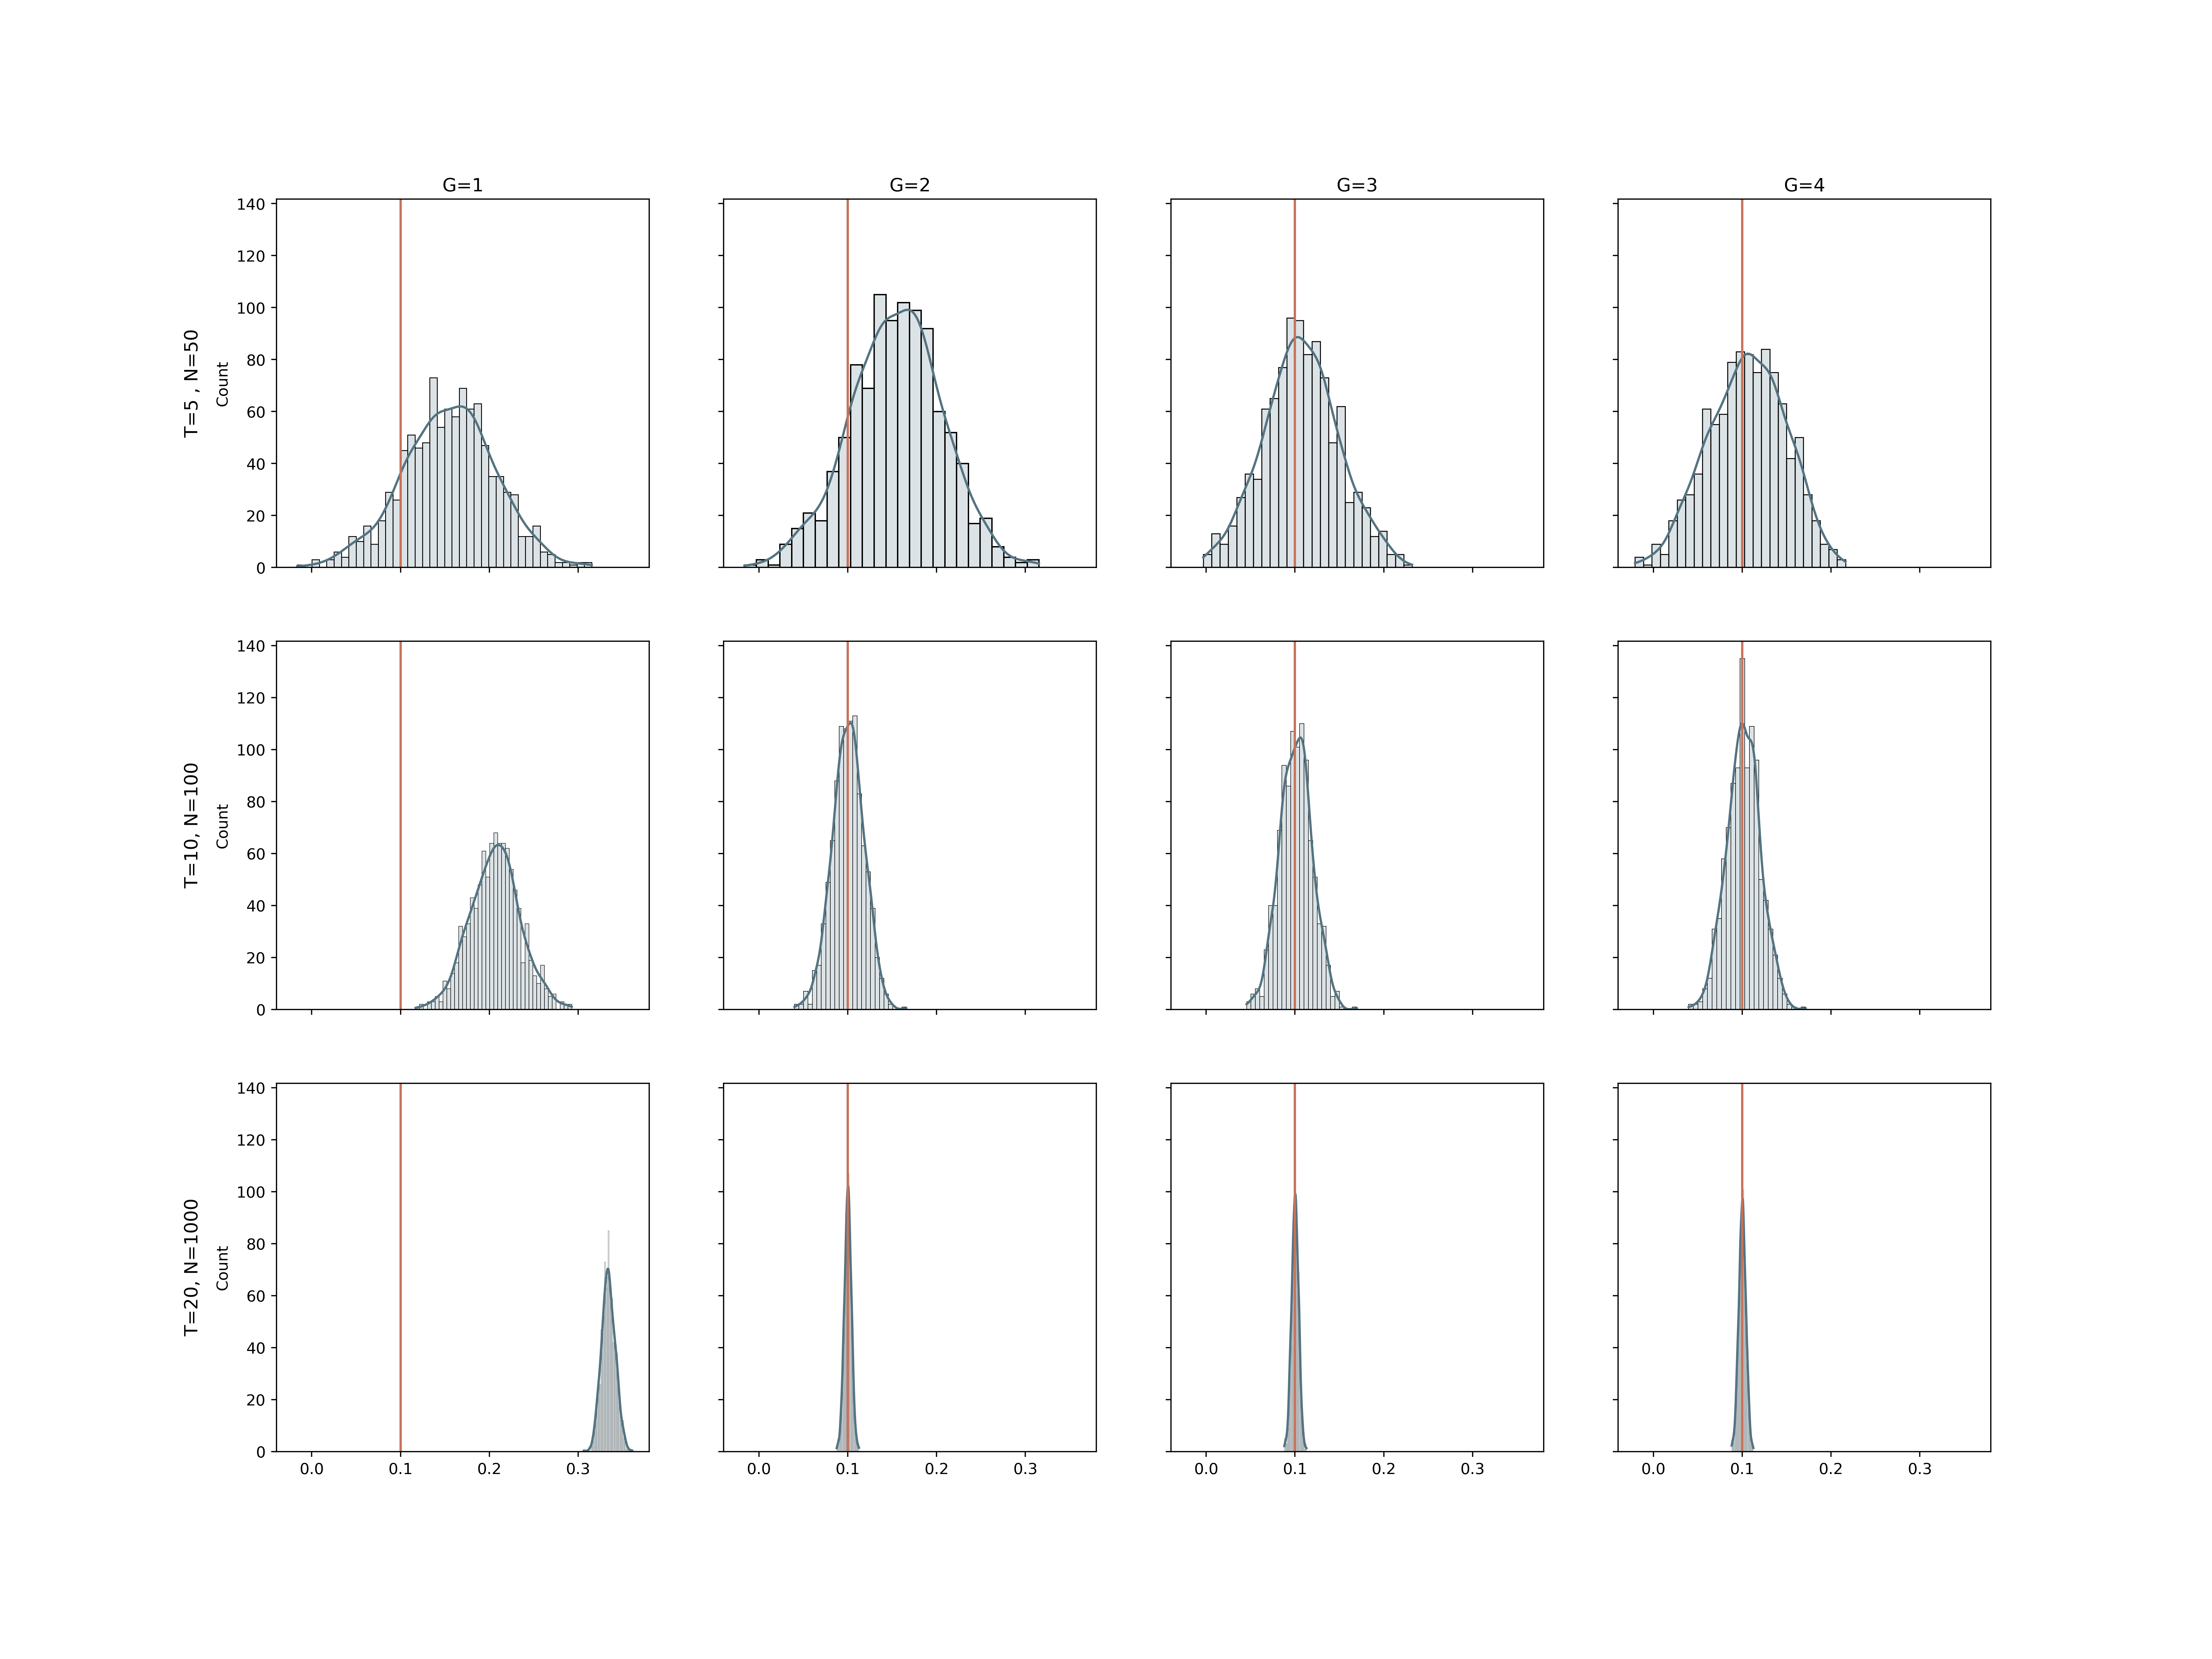
\includegraphics[scale=0.31]{figures/groupssamplingplot1.png}
\end{flushleft}
\caption{Sampling Distribution of $\hat{\theta_1}$ when both T and N increases in different number of group specifications where $G^0 = 2$.}
\label{fig:gs}
\end{figure}

Figure \ref{fig:gsn} is aimed to show the consistency of the GFE estimates of $\theta_2$ which its corresponding regressor is nonlinearly correlated with the grouped-fixed effects. The sampling distribution when both T and N increases. The last row again shows the estimates of G=1 is biased and inconsistent. While G=2,3,4, where $G^0=2$ is consistent.

\begin{figure}[h]
\begin{flushleft}
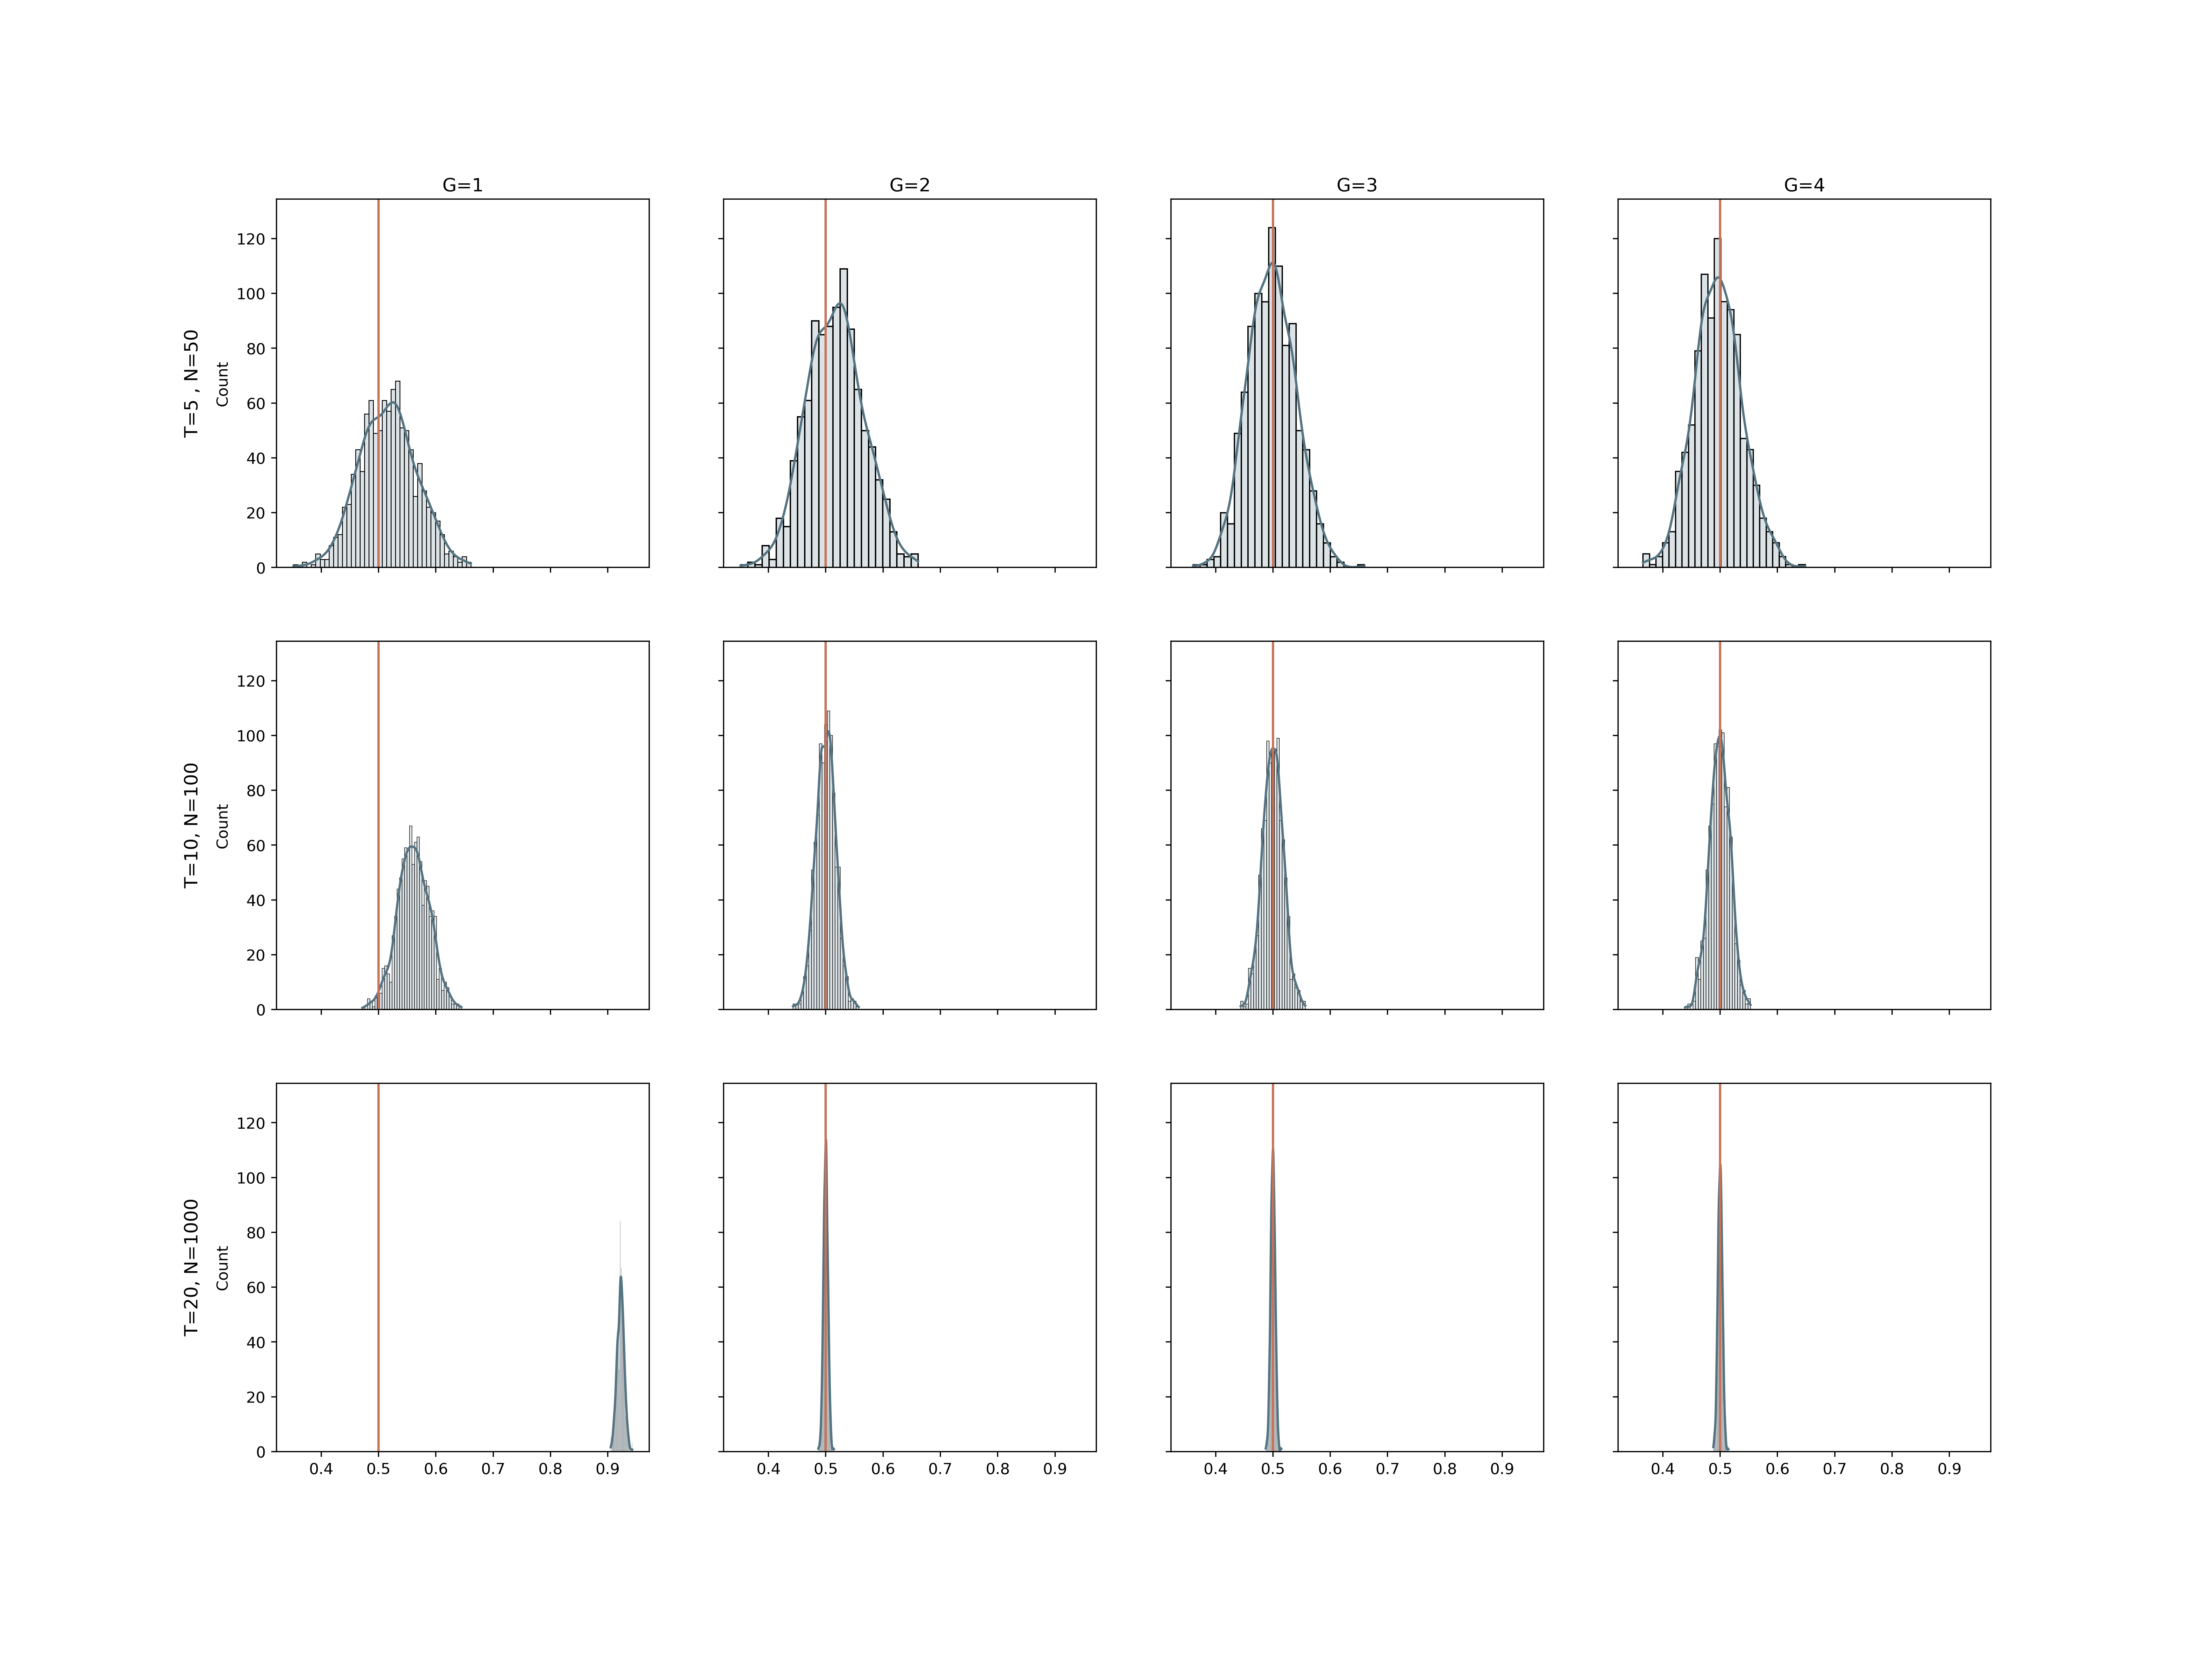
\includegraphics[scale=0.31]{figures/groupssamplingplot.png}
\end{flushleft}
\caption{Sampling Distribution of $\hat{\theta_2}$ when both T and N increases in different number of group specifications where $G^0 = 2$.}
\label{fig:gsn}
\end{figure}

Intuition from OLS suggests that including an irrelevant regressor do not effect the asymptotic properties of the estimator. Nevertheless, some finite sample inefficiency is expected. Before looking at the finite sample properties of the GFE estimator where the number groups are misspecified, we look at how the individuals are divided into groups and how the additional $\hat{\alpha}$ are estimated for some intuition.

Figure \ref{fig:staringalphas} shows the starting value of $\alpha$ for specified number of groups of G=1,2,3,4. For G=2, the true value of $\alpha$ is used as the starting value in Figure \ref{fig:staringalphas}.

\begin{figure}[h!]
\centering
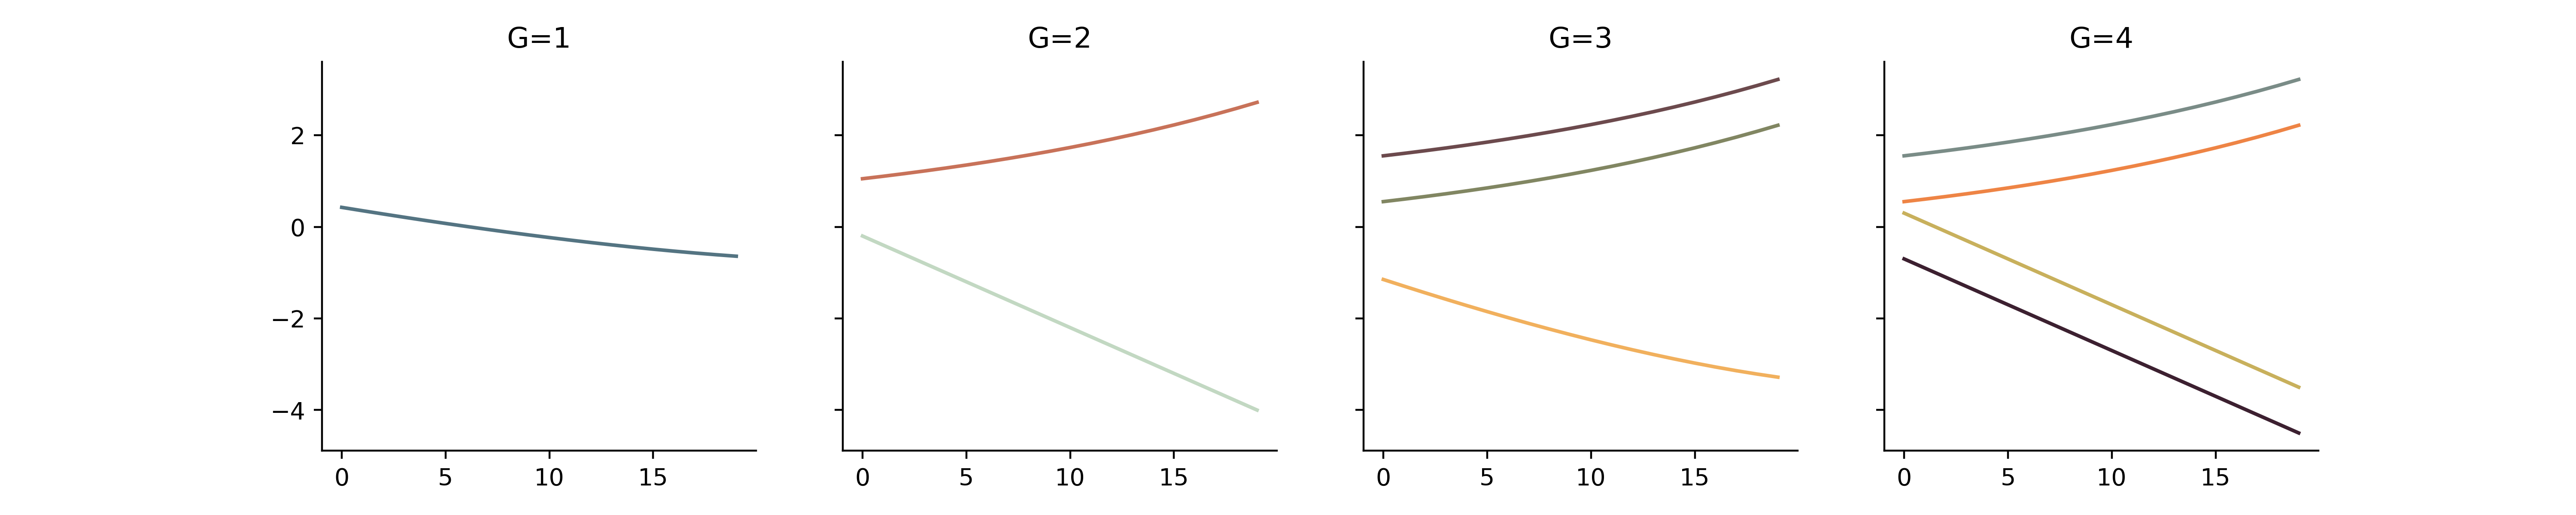
\includegraphics[scale=0.4]{figures/startingvalues.png}
\caption{$\alpha^{(0)}$ in Algorithm 1}
\label{fig:staringalphas}
\end{figure}

Specification $G=1$ basically introduces time dummies into the regression and does not account for the group structure leading to an omitted variable bias. We can think of it as as allowing only for $\xi_t$ and assuming $c_i, \lambda_i' f_t, \alpha_{gt} = 0$ in the context of the theoretical background. 
To contrasts, specification $G=2$ shows and accounts for the grouped patterns of heterogeneity in the data. Specification $G=3$ and $G=4$ divides the groups into subgroups and fits group heterogeneity with parts of idiosyncratic error term. They introduce additional group-time dummies into the regression. The added fit of over specified groups comes from the idiosyncratic error term that is irrelevant for the causal effect. However, the $\hat{\alpha}_{G>G^0}$ estimates added by number of group overspecification account for both the grouped patterns of heterogeneity and the idiosyncratic error as the individuals divided into more groups. When the number of groups are overspecified inference is not possible for $\hat{\alpha}_{G>G^0}$. Relating to Remark 4 in \textcite{bai2009panel} on p. 1247, some efficiency loss is expected.

Table \ref{tab:table2} reports on bias, RMSE and CP of the GFE estimator with different number of groups specifications. The results show that $G \leq G^0$ is inadequate. On the other hand when $G \ge G^0$, the coverage probabilities stays comparable and close to $G = G^0$. Unlike IFE in \ref{tab:table0} where the overfitting decreased the bias and increased the variance. The bias and RMSE of $G \ge G^0$ is remains similar with minor differences to $G = G^0$ for each N and T suggesting a similarity in their asymptotic distribution. 

\begin{table}[p]
    \centering
    \begin{tabular}{lll|ccc|ccc}
\toprule
   &      &   &       &  $\hat{\theta_1}$   &             &    & $\hat{\theta_2}$ & \\
   \hline
T & N & G & Bias &    RMSE       &      CP     &    Bias &    RMSE       &      CP           \\
\midrule
5  & 50   & 1 &  0.054515 &  0.075302 &                 0.774 & 0.016464 &  0.052199 &                 0.924 \\
   &      & 2 &  0.054515 &  0.075302 &                 0.609 & 0.016464 &  0.052199 &                 0.817 \\
   &      & 3 &  0.007147 &  0.042757 &                 0.874 &-0.001957 &  0.041414 &                 0.895 \\
   &      & 4 &  0.005630 &  0.043443 &                 0.852 &-0.003852 &  0.042086 &                 0.864 \\
   & 100  & 1 &  0.053953 &  0.065008 &                 0.639 & 0.016095 &  0.037208 &                 0.938 \\
   &      & 2 &  0.002530 &  0.028159 &                 0.923 &-0.000581 &  0.026704 &                 0.945 \\
   &      & 3 &  0.005137 &  0.031111 &                 0.880 &-0.001322 &  0.028468 &                 0.907 \\
   &      & 4 &  0.004068 &  0.030487 &                 0.864 &-0.002602 &  0.029530 &                 0.880 \\
   & 1000 & 1 &  0.054041 &  0.055140 &                 0.001 & 0.015190 &  0.018637 &                 0.713 \\
   &      & 2 &  0.002218 &  0.008892 &                 0.921 & 0.000372 &  0.008639 &                 0.932 \\
   &      & 3 &  0.004243 &  0.010095 &                 0.865 & 0.000682 &  0.009194 &                 0.909 \\
   &      & 4 &  0.002963 &  0.009841 &                 0.870 & 0.000414 &  0.009327 &                 0.896 \\
10 & 50   & 1 &  0.105206 &  0.112956 &                 0.264 & 0.059915 &  0.072625 &                 0.686 \\
   &      & 2 & -0.000390 &  0.027524 &                 0.929 &-0.000520 &  0.025941 &                 0.955 \\
   &      & 3 &  0.000526 &  0.028568 &                 0.910 &-0.001678 &  0.026467 &                 0.945 \\
   &      & 4 &  0.002240 &  0.029164 &                 0.903 &-0.002827 &  0.027290 &                 0.917 \\
   & 100  & 1 &  0.106493 &  0.110116 &                 0.038 & 0.060961 &  0.067022 &                 0.455 \\
   &      & 2 &  0.000420 &  0.017785 &                 0.954 & 0.000179 &  0.017274 &                 0.958 \\
   &      & 3 &  0.001118 &  0.018308 &                 0.941 &-0.000121 &  0.018026 &                 0.941 \\
   &      & 4 &  0.001640 &  0.018908 &                 0.924 &-0.000780 &  0.017871 &                 0.940 \\
   & 1000 & 1 &  0.105803 &  0.106192 &                 0.000 & 0.059296 &  0.059985 &                 0.000 \\
   &      & 2 &  0.000307 &  0.005713 &                 0.955 & 0.000282 &  0.005541 &                 0.955 \\
   &      & 3 &  0.000304 &  0.005857 &                 0.950 & 0.000269 &  0.005664 &                 0.946 \\
   &      & 4 &  0.000339 &  0.005970 &                 0.934 & 0.000150 &  0.005745 &                 0.938 \\
20 & 50   & 1 &  0.238163 &  0.240944 &                 0.000 & 0.429078 &  0.430069 &                 0.000 \\
   &      & 2 &  0.000512 &  0.017937 &                 0.957 & 0.000251 &  0.017497 &                 0.959 \\
   &      & 3 &  0.001167 &  0.018181 &                 0.942 &-0.000483 &  0.017839 &                 0.949 \\
   &      & 4 &  0.001947 &  0.018758 &                 0.939 &-0.001245 &  0.018226 &                 0.944 \\
   & 100  & 1 &  0.235297 &  0.236822 &                 0.000 & 0.424235 &  0.424768 &                 0.000 \\
   &      & 2 &  0.000265 &  0.013012 &                 0.946 & 0.000533 &  0.013551 &                 0.932 \\
   &      & 3 &  0.000630 &  0.013289 &                 0.945 & 0.000072 &  0.013842 &                 0.929 \\
   &      & 4 &  0.001156 &  0.013439 &                 0.935 &-0.000434 &  0.014113 &                 0.921 \\
   & 1000 & 1 &  0.234128 &  0.234257 &                 0.000 & 0.422433 &  0.422477 &                 0.000 \\
   &      & 2 &  0.000160 &  0.003963 &                 0.954 & 0.000003 &  0.003857 &                 0.962 \\
   &      & 3 &  0.000167 &  0.004001 &                 0.951 & 0.000003 &  0.003884 &                 0.964 \\
   &      & 4 &  0.000193 &  0.004069 &                 0.943 &-0.000039 &  0.003911 &                 0.955 \\
\bottomrule
\end{tabular}

    \caption{Simulation: GFE Group Specification} %subject to change
    \label{tab:table2}
\end{table}

Figure \ref{fig:cilength} shows the average confidence intervals of the GFE estimators with different number of groups specifications for $\theta_1 = 0.10$. The average is taken over 1000 replications when T=10, N=100. The horizontal blue dotted line marks the true, black dots are the mean of the $\theta_1$ estimates for the given estimator with the number of groups specification stated in x-axis. The confidence intervals overlap when $G \geq G^0$. 
\begin{figure}[h]
\centering
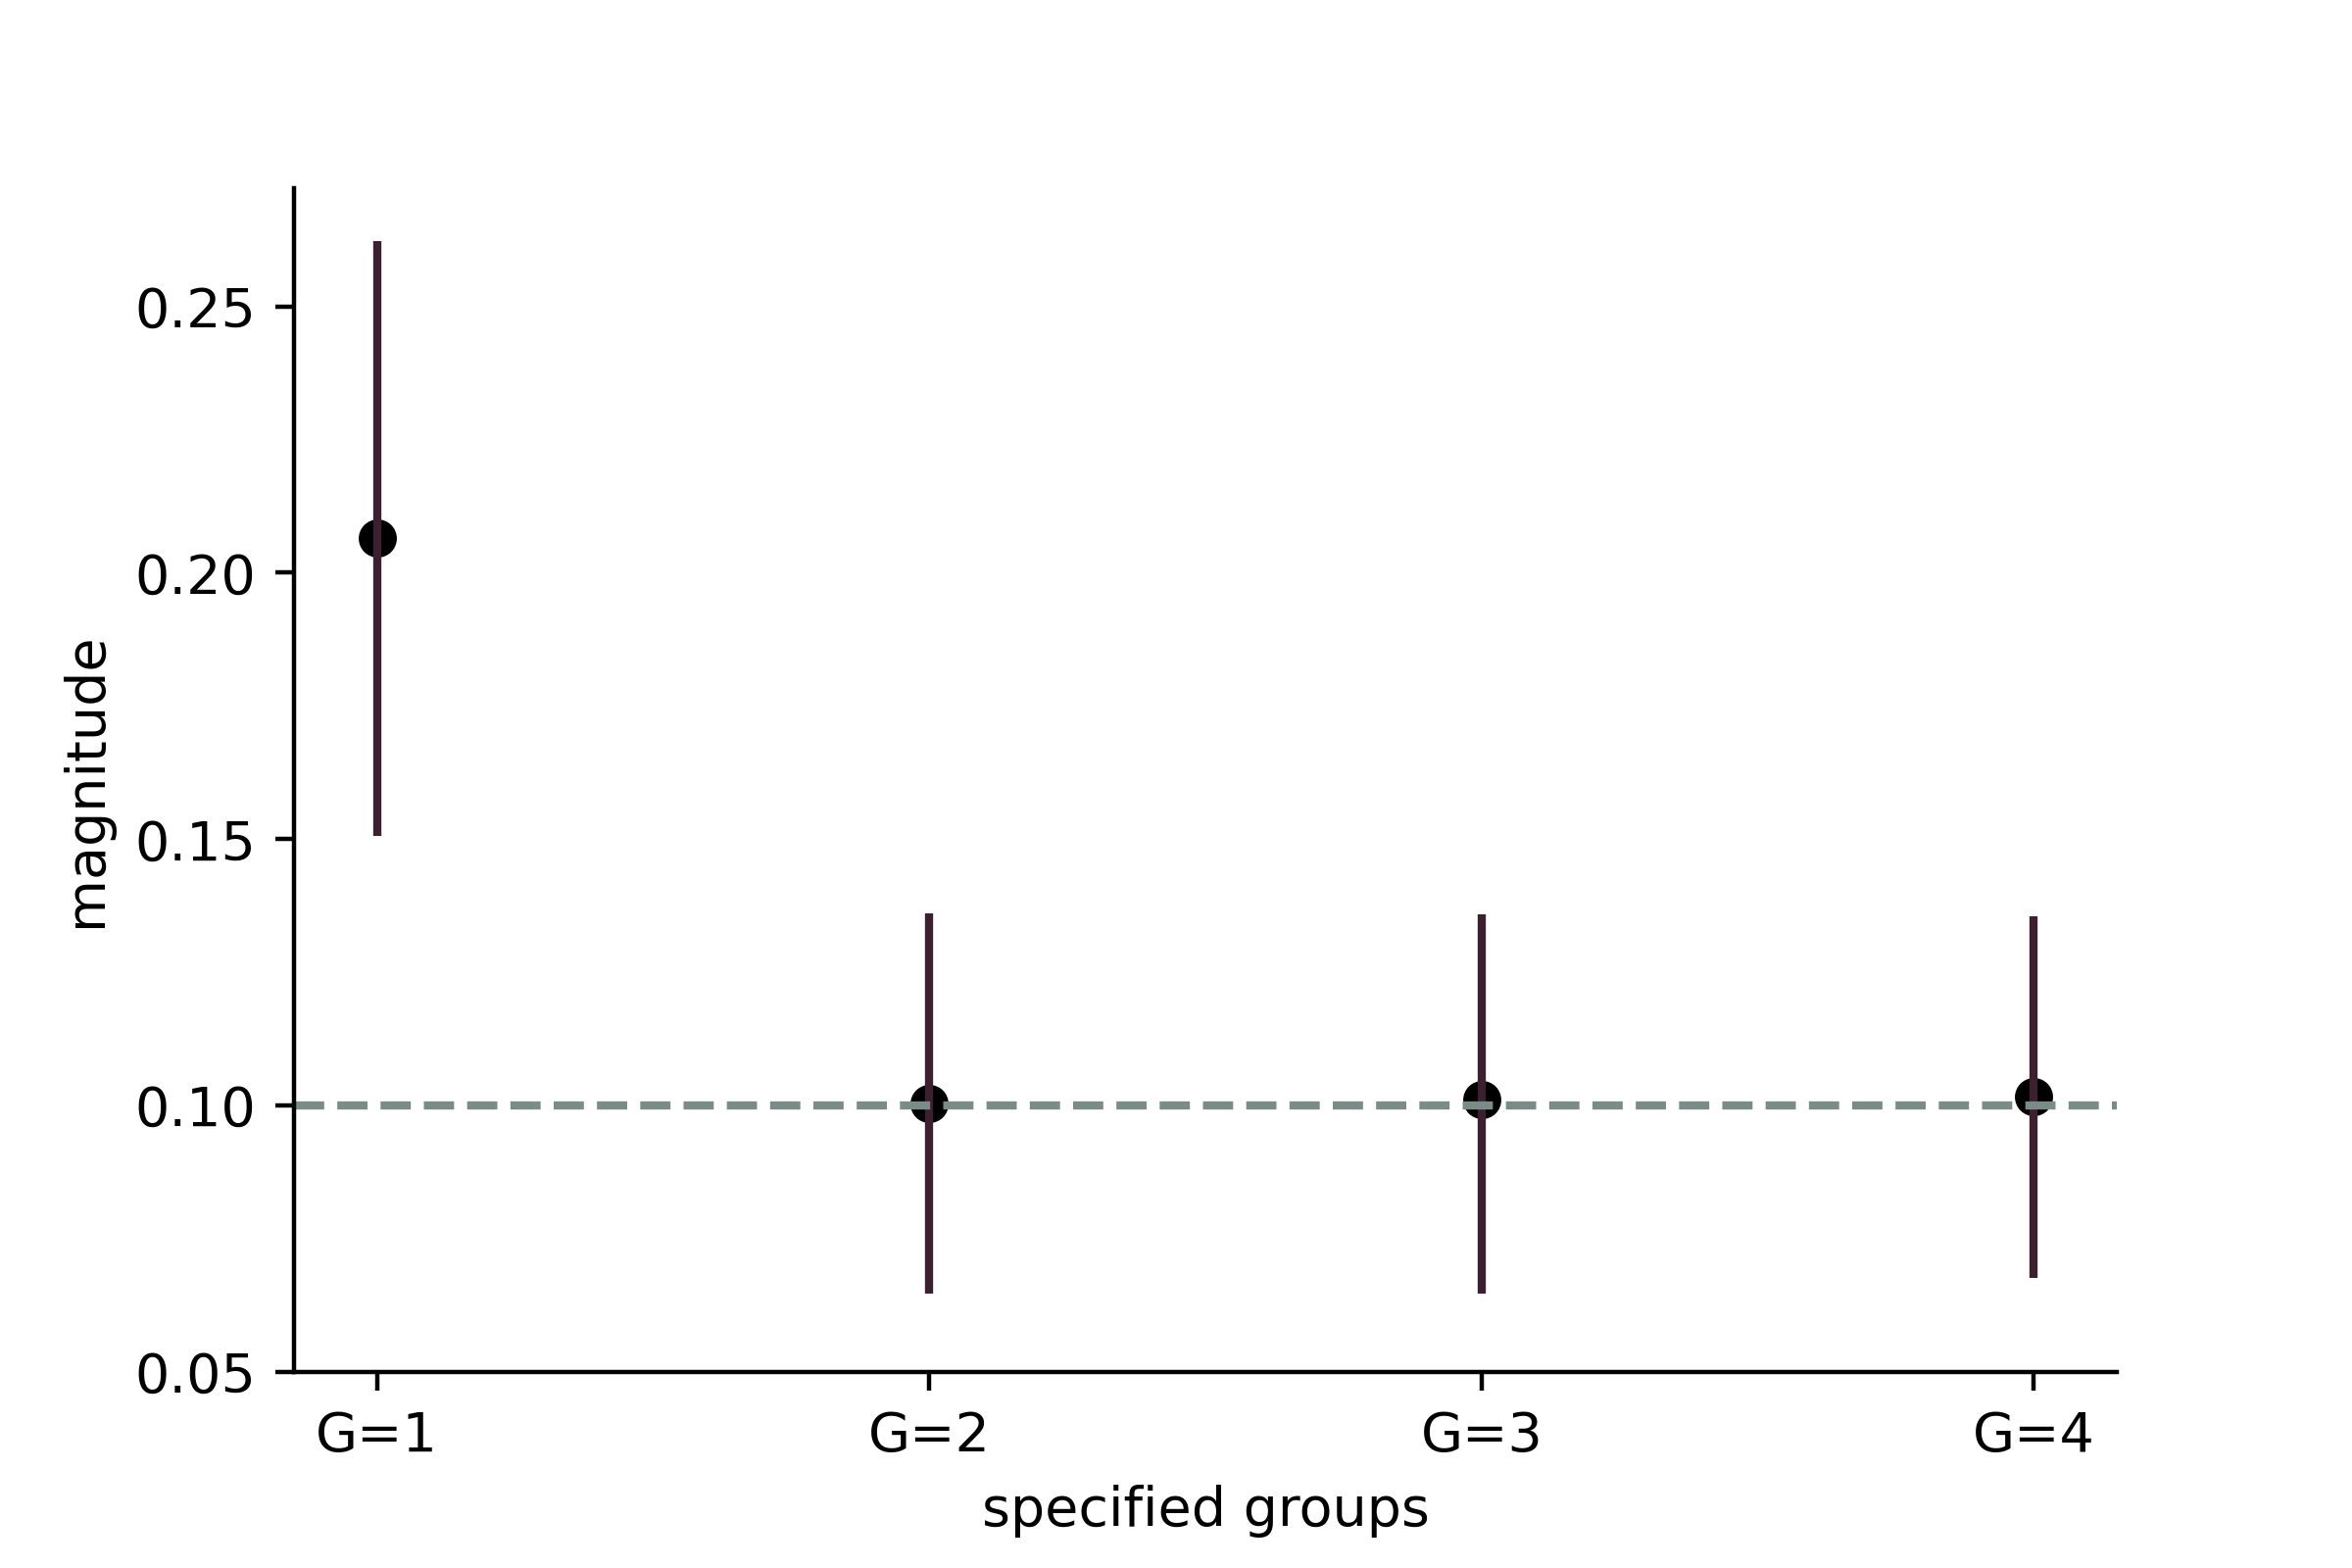
\includegraphics[scale=0.85]{figures/ciplot.png}
\caption{Expected Value and Average Confidence Intervals of $\hat{\theta}_1$ T=10, N=100.}
\label{fig:cilength}
\end{figure}
 
Finite sample properties important because it shows how the model perform in application and for inference. 


%\footnote{Model is estimated using the package in: https://github.com/FixedEffects/InteractiveFixedEffectModels.jl}

%in less precise results. Even though it does not lead to a bias and the overspecified estimator is still consistent, it has higher asymptotic variance, therefore, less efficient and less precise. It is expected that the overspecification leads to some finite sample inefficiencies. Before looking at the finite sample properties, we try to We begin by looking at the starting value of $\alpha$ for different number of groups from which we will draw heuristics.

\subsection{Evaluation of the Computation Method of GFE} \label{section:sensitivity}
\paragraph{Sensitivity.} The iterative algorithm described in subsection \ref{section:algo} depends on the starting values influencing whether the algorithm converges to a local minima or the global minima.Practical solution suggested by \textcite{bonhomme2015grouped} for low dimensional problems is to drawing starting values at random and selecting the solution yielding the lowest objective. This additional procedure increases the computational time of the algorithm significantly.It has not been implemented due to time constraints and to shorten the amount of time the simulations take. However, to ensure the quality of the results of my implementation, the sensitivity to starting values has been studied.

In the simulation tests for the sensitivity to starting values, the algorithm was insensitive to values of $\theta^{(0)}$ given a reasonable value is chosen\footnote{Extreme cases such as $\theta^{(0)}$ is outside the range of the outcome variable is not tested}. In contrast, it is sensitive to $\alpha^{(0)}$ values. 
Given the DGP in subsection \ref{section:DGP}, diverting the true $\alpha$ values up to a 0.1 change, results in 24 percent of different objective functions and thus different estimates. The mean of $\hat{\theta}$ estimates from 100 simulation runs is different only after the third decimal point such. The tests also show that using starting values does not necessarily lead to the global minima.  

The starting values for different groups should be also well separated in order to avoid singular matrix problems occurring when the solution algorithm has an empty group and the GFE estimates are not identified. This has been a prominent issue in earlier simulation runs.How much variation in error term the algorithm and the estimator allows worth further attention. \textcite{bonhomme2015grouped} suggest as a solution to assign one random individual into the empty group which decreases the objective function.

\paragraph{Computational performance in comparison to other methods.}
I used existing established packages for the remaining methods. The computation was fastest for OLS but followed up by GFE and slowest for IFE. Nevertheless, it should be noted that established packages runs various checks and often compute a regression table with statistics that are not always needed for the simulation results. 

The code of my implementation of the estimator, simulations, and the additional results which are omitted here can be found on: \href{https://github.com/baharcos/gfe.}{github.com/baharcos/gfe}.








\section{Conclusion}\label{conclusion}
This paper studies the theoretical properties of a set of well-established panel models compared to the novel GFE model.  All estimators impose a different set of assumptions on the data. The GFE which is the main focus of this paper, is a flexible approach, well-adapted to account for clustered unobserved heterogeneity impacting regressors and the dependent variable. GFE's assumptions include small unobserved individual heterogeneity within groups and a known number of groups. 
Simulations compare the methods discussed in the theoratical part when a grouped pattern of unobserved heterogeneity exists. A tailored DGP for GFE looks at its finite sample properties compared to well-established methods. 

After establishing the validity of employing GFE model, a more detailed simulation study is conducted for GFE estimator with misspecified groups. I provide heuristics on model selection from OLS and IFE. 
Simulation results do not suffer from large finite sample inefficiencies when the number of groups are overspecified. This suggests the inference on common parameters is still possible with overspecified groups. Even though grouped-fixed effect estimates suffer from large biases.

The similar finite sample properties of GFE with overspecified number of groups and GFE estimator with true number of groups suggest a possibility for asymptotic equivalence of the two estimator. Showing the asymptotic equivalence of the GFE estimator with overspecified number of groups and GFE estimator with true number of groups pose  a challenge and an interesting question for future research econometric theory.



\newpage

\printbibliography[heading=bibintoc,title={References}] 

\newpage

\setcounter{figure}{0} 
\renewcommand{\thefigure}{A.\arabic{figure}}
\setcounter{table}{0} 
\renewcommand{\thetable}{A.\arabic{table}}
\setcounter{equation}{0} \renewcommand{\theequation}{A.\arabic{equation}}
\setcounter{footnote}{0}

\pagenumbering{Roman}
\renewcommand{\thesection}{A}
\section{Appendix}
GFE $\theta$ estimates are root-N consistent.

\begin{figure}[h]
\begin{flushleft}
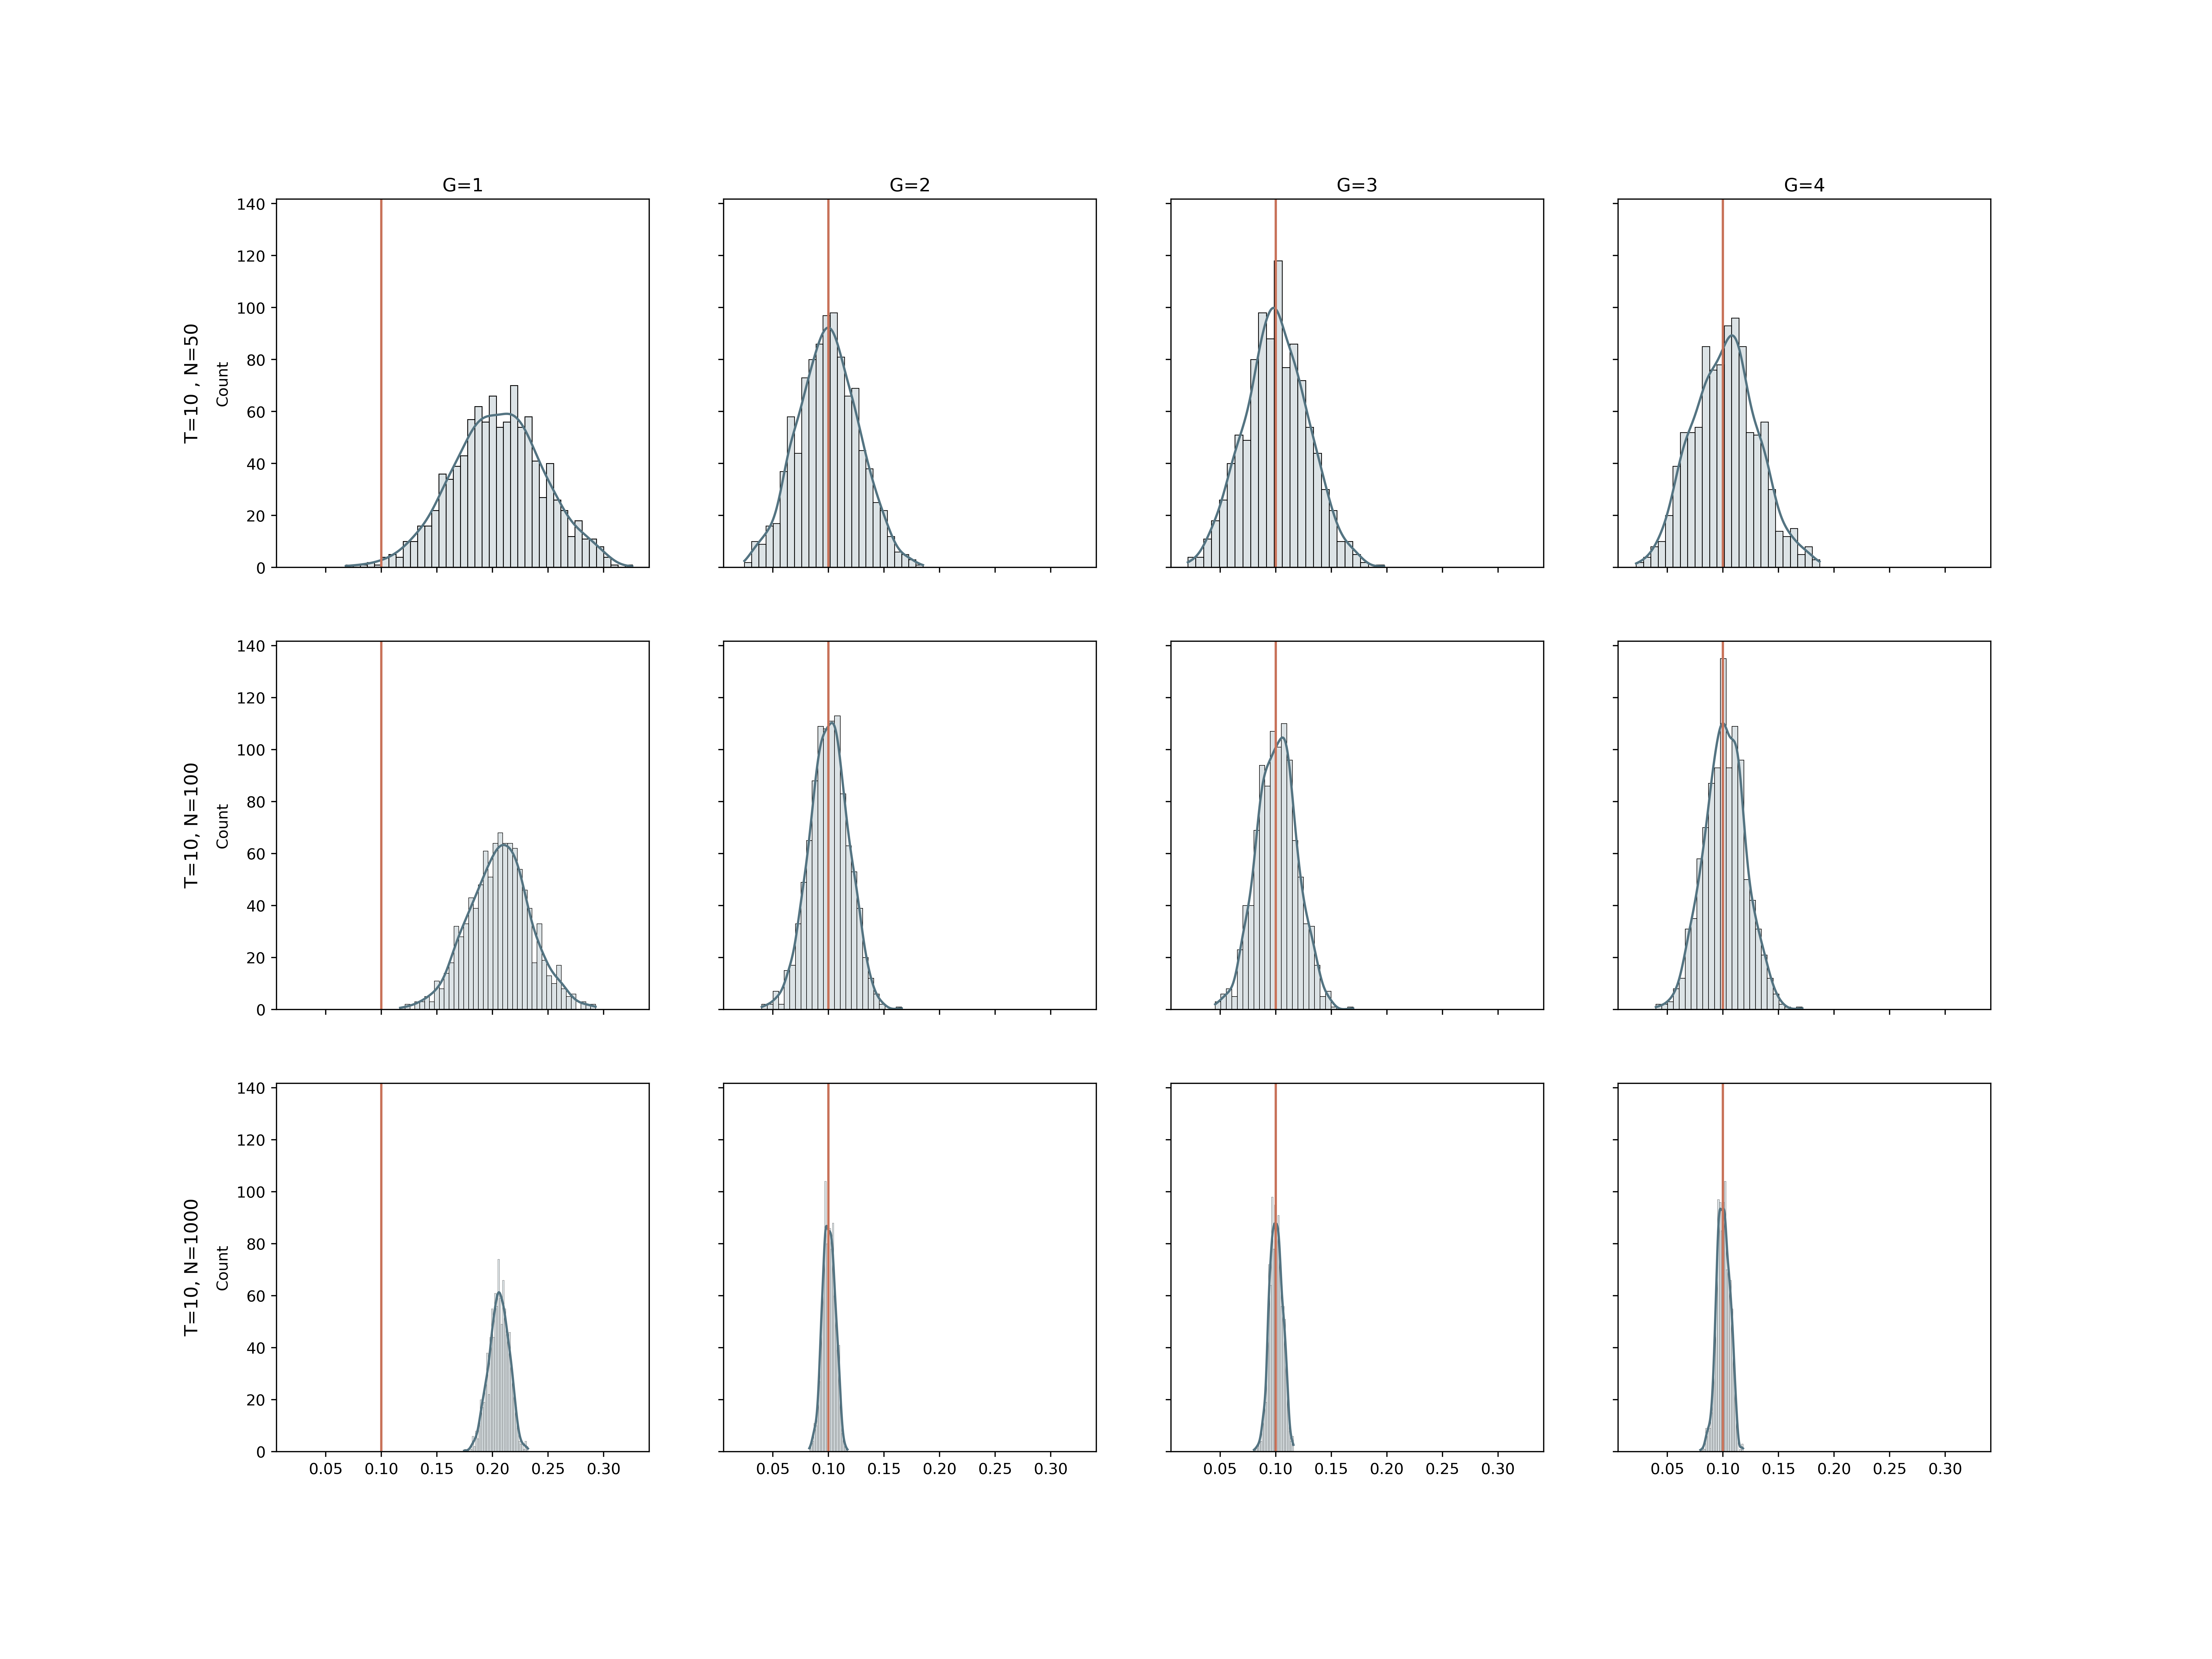
\includegraphics[scale=0.31]{sections/appendix/groupssamplingplotN1.png}
\end{flushleft}
\caption{Sampling Distribution of $\hat{\theta_1}$ when T=10 and N increases in different number of group specifications where $G^0 = 2$.}
\label{fig:gsn}
\end{figure}

\begin{figure}[h]
\begin{flushleft}
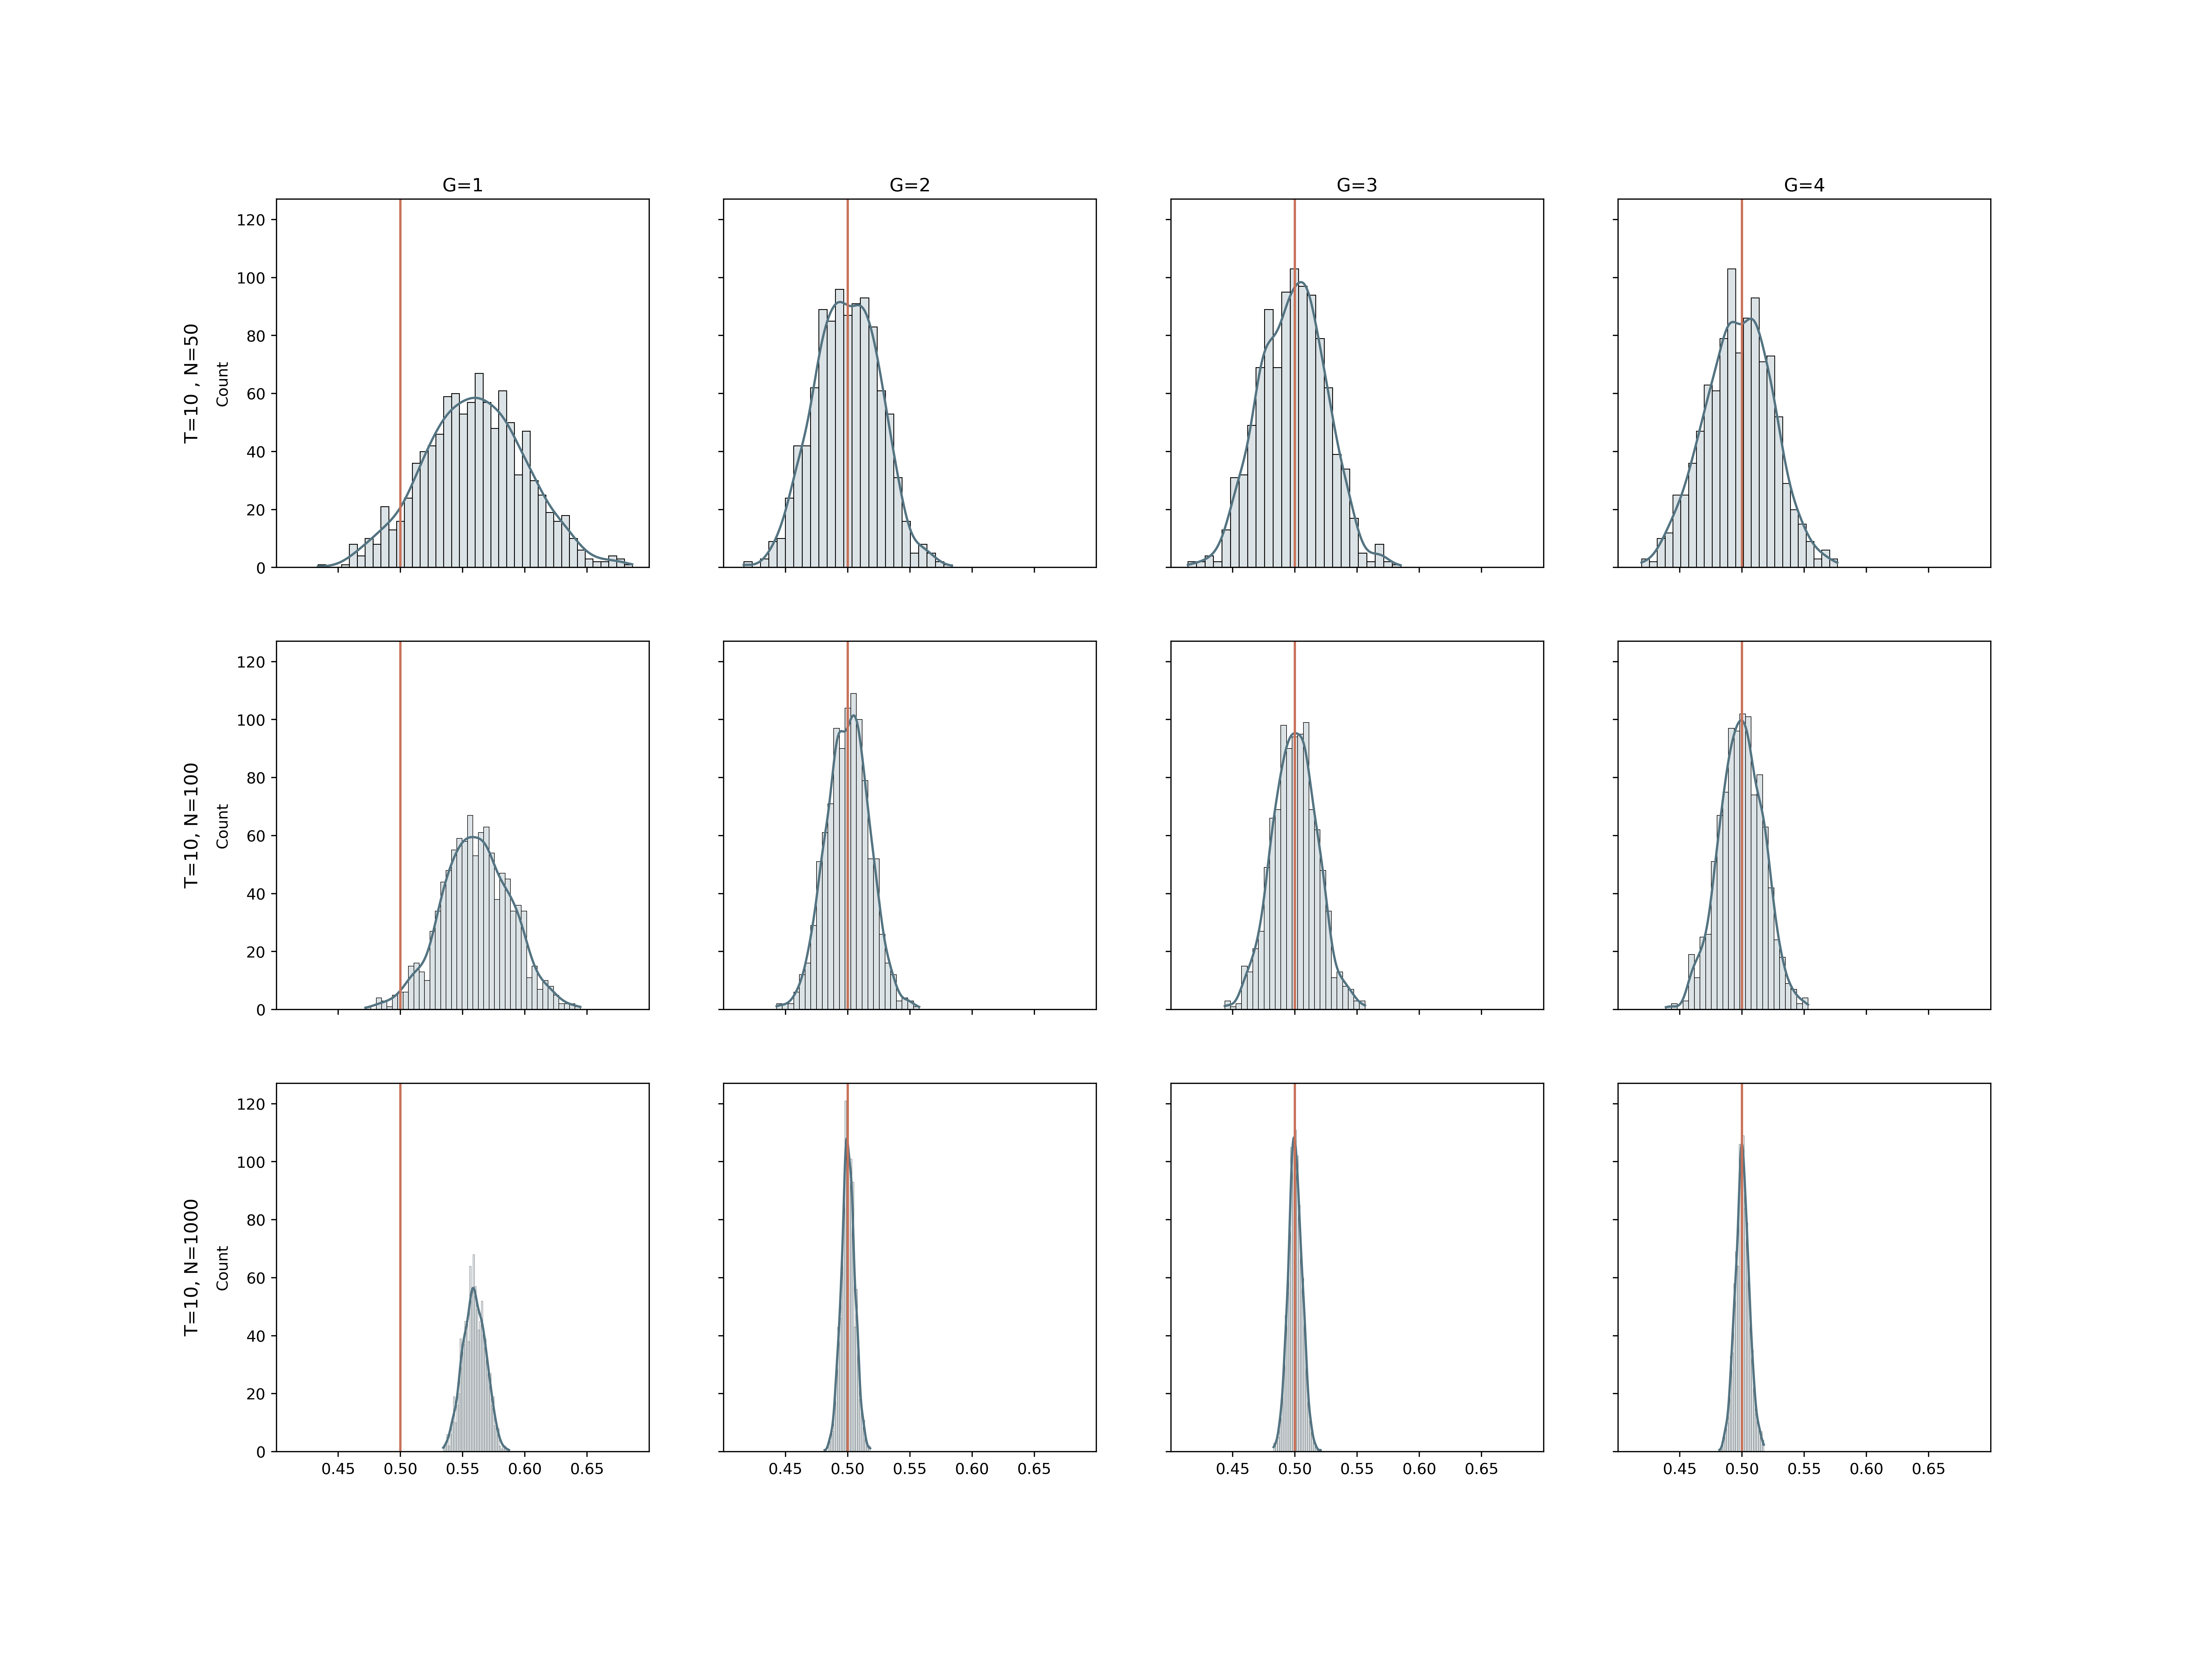
\includegraphics[scale=0.31]{sections/appendix/groupssamplingplotN.png}
\end{flushleft}
\caption{Sampling Distribution of $\hat{\theta_2}$ when T=10 and N increases in different number of group specifications where $G^0 = 2$.}
\label{fig:gsn}
\end{figure}

\begin{figure}[h]
\begin{flushleft}
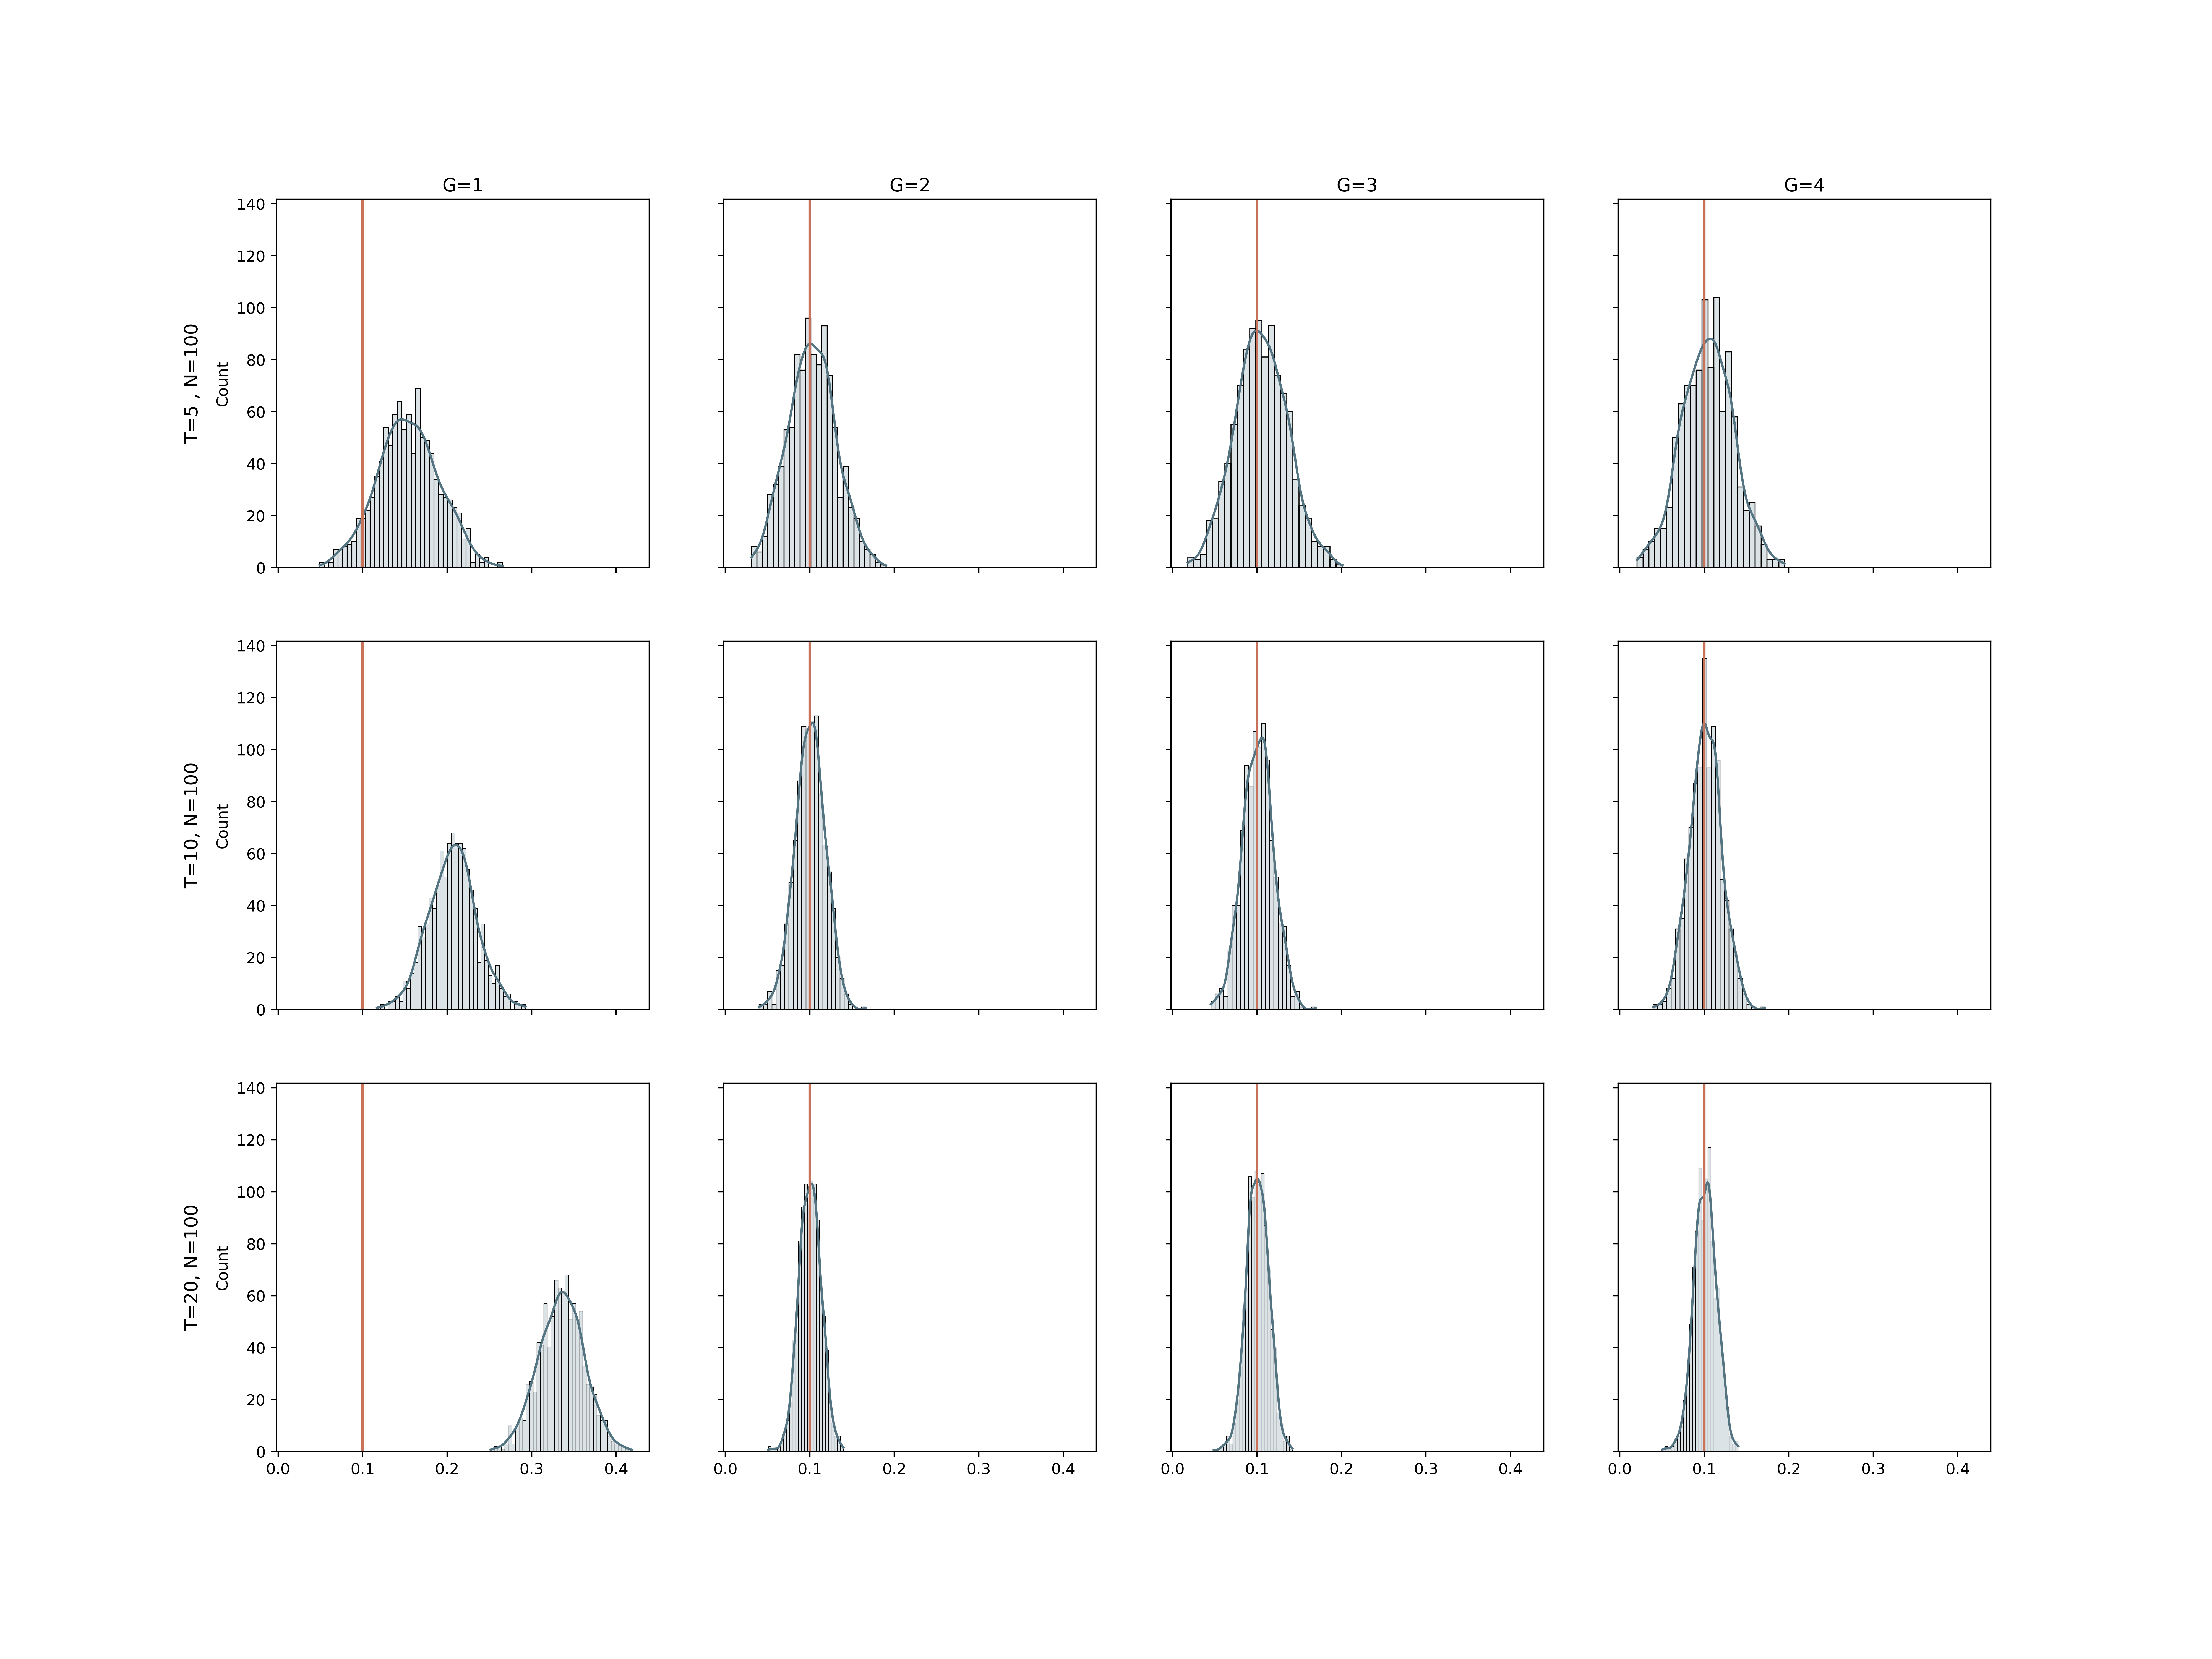
\includegraphics[scale=0.31]{sections/appendix/groupssamplingplotT1.png}
\end{flushleft}
\caption{Sampling Distribution of $\hat{\theta_1}$ when N=100 and T increases in different number of group specifications where $G^0 = 2$.}
\label{fig:gsn}
\end{figure}

\begin{figure}[h]
\begin{flushleft}
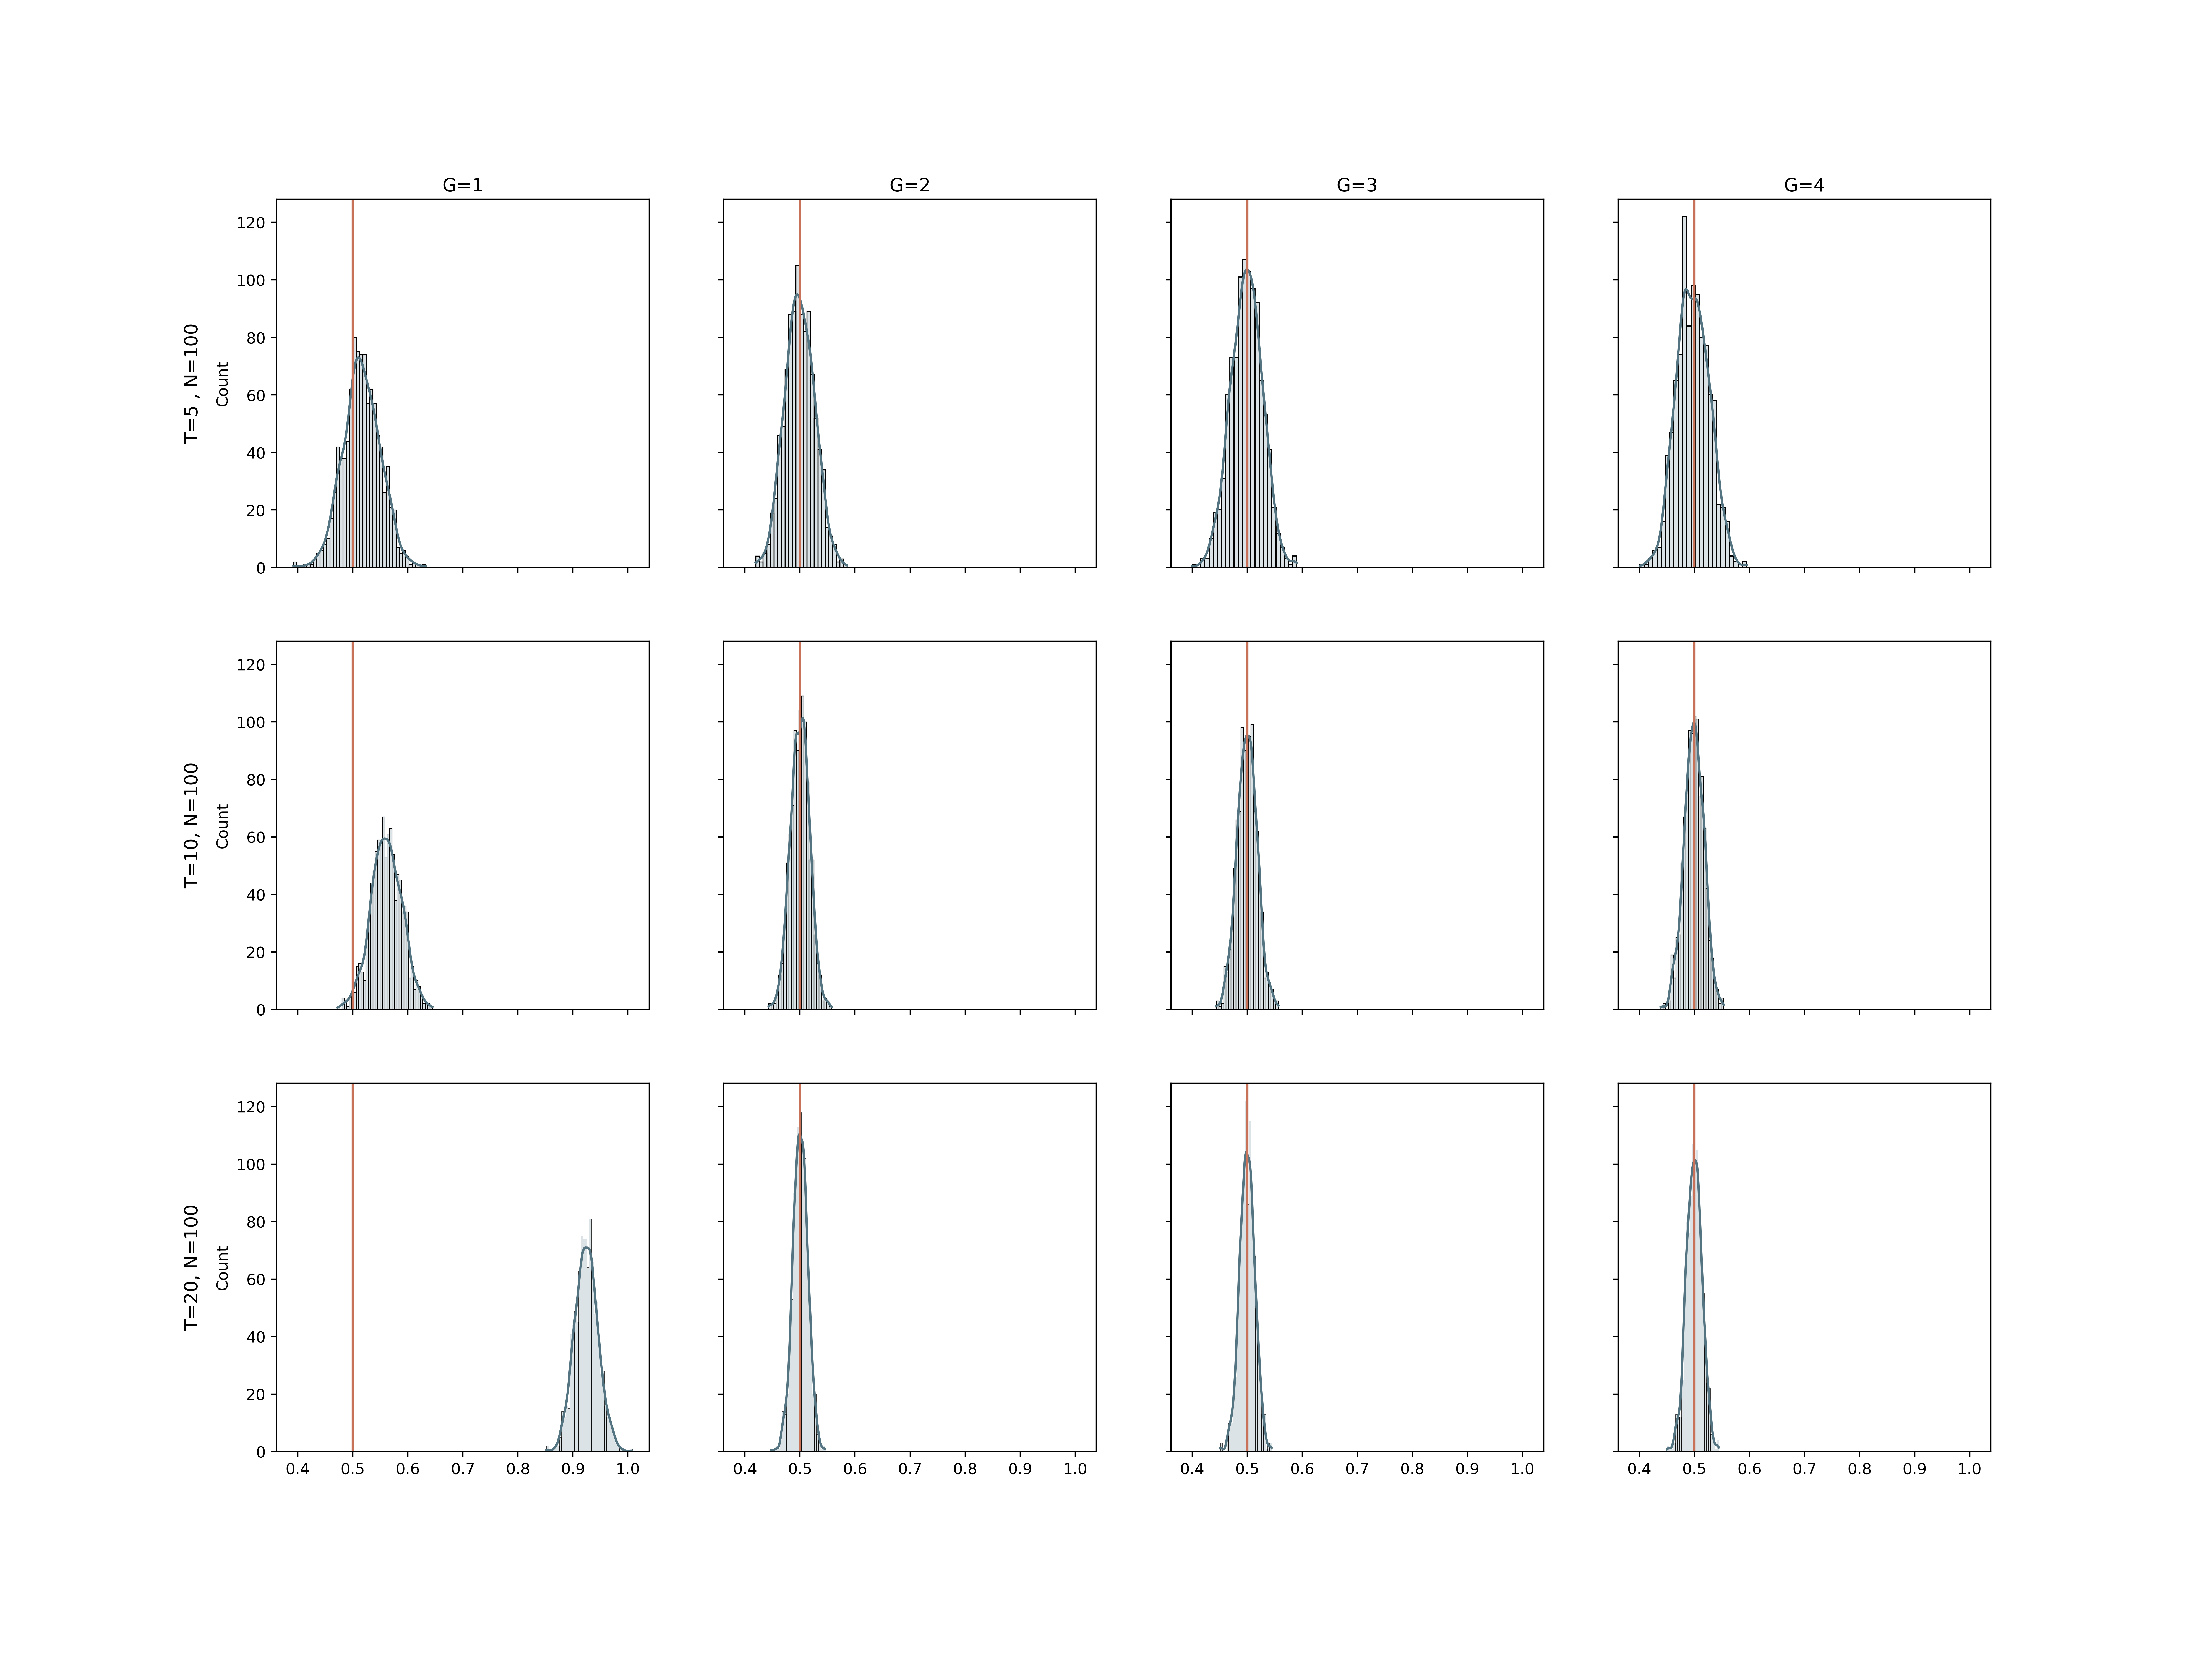
\includegraphics[scale=0.31]{sections/appendix/groupssamplingplotT.png}
\end{flushleft}
\caption{Sampling Distribution of $\hat{\theta_2}$ when N=100 and T increases in different number of group specifications where $G^0 = 2$.}
\label{fig:gsn}
\end{figure}



\begin{figure}[h]
\begin{center}
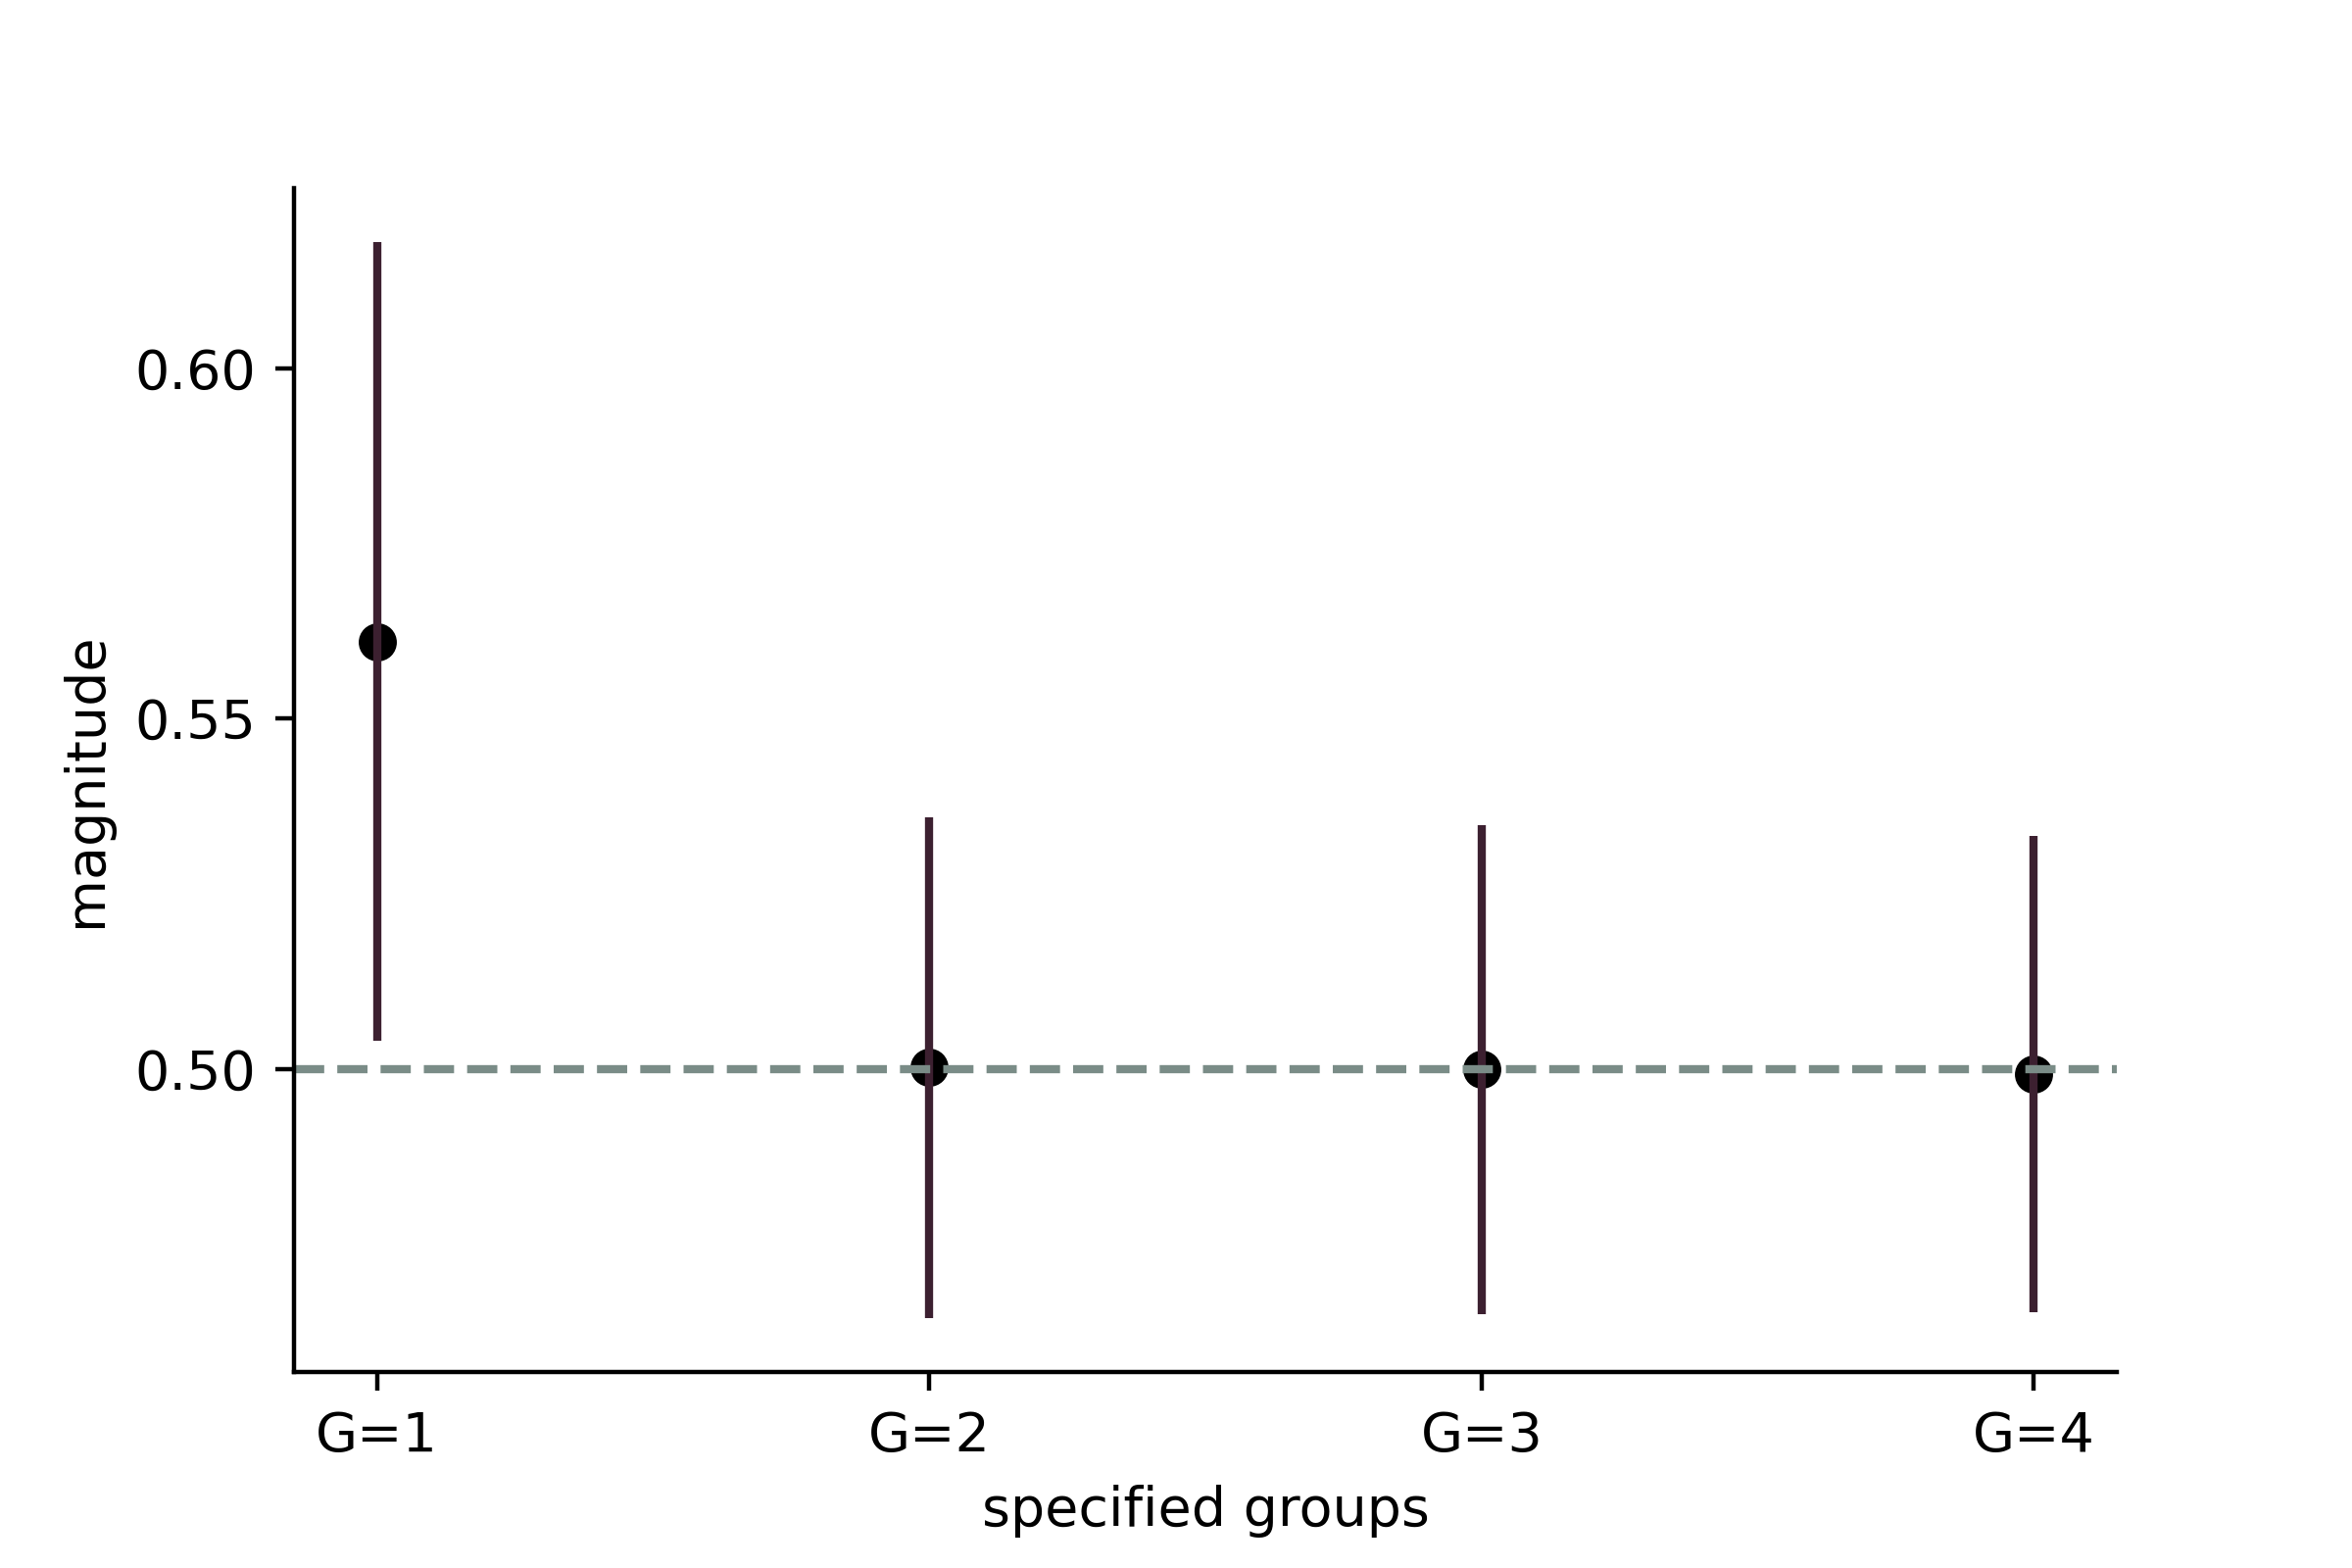
\includegraphics[scale=0.85]{sections/appendix/ciplottheta2.png}
\end{center}
\caption{Expected Value and Average Confidence Intervals of $\hat{\theta}_2$, T=10, N=100.}
\label{fig:ci2}
\end{figure}


%Proofs of WLLN and CLT are omitted.
%\subsection{Weak Law of Large Numbers}
%How to cite? My source here are chapter 4 of Michael's Econometric Basic Module WS 19/20 notes and Joachim's 5th handout of Econometrics I WS 19/20 which is from Casella and Berger (2001), Section 5.5..

Suppose $\{X_1, \dots, X_n\}$ is a sequence of i.i.d. $\mathbb{R}^k$ valued random variables  i.e. a random sample from a distribution.
Let $\Bar{X}_n$ denote the sample mean $\dfrac{1}{N}\sumi X_i$ and $\EX(X_n)$ exists then $\Bar{X}_n \overset{p}{\to} \EX(X_n)$. 

In the case where $X_i$ and $X_j$ for $i \neq j$ is not independent
but uncorrelated random variables, we would additionally need to assume existence of the variance to get this result.


\subsection{Central Limit Theorem}

Suppose $\{X_1, \dots, X_n\}$ is a sequence of i.i.d. $\mathbb{R}^k$ valued random variables and suppose $\EX(X_n) = \mu$ and $Cov(X_n)= \Sigma$ exists, then $\sqrt{n}(\Bar{X}_n - \mu) \sim \mathcal{N}(0,\Sigma)$.

\subsection{Continuous Mapping Theorem}

Suppose $\{X_1, \dots, X_n\}$ is a sequence of i.i.d. $\mathbb{R}^k$ valued random variables and g: $\mathbb{R}^k \rightarrow \mathbb{R} $ is a continuous function:
\begin{itemize}
    \item If $X_n \overset{p}{\to} X$ then  $g(X_n) \overset{p}{\to} g(X)$.
    \item If $X_n \overset{d}{\to} X$ then  $g(X_n) \overset{d}{\to} g(X)$.
\end{itemize}


%\subsection{Proof of Theorem 2.1: Consistency of Pooled OLS}

Under assumption $\mathcal{P}$, $\hat\theta_{pool}$ is identified as:
\begin{align*}
    \hat\theta_{pool} = (\sumt \sumi  x_{it}x_{it}')^{-1}\sumi\sumt x_{it}y_{it}
\end{align*}
When we plug in the model $y_{it} =  x_{it}'\theta + e_{it}$:

\begin{align*}
    \hat\theta_{pool} = (\sumt \sumi x_{it}x_{it}')^{-1}\sumt\sumi x_{it}x_{it}'\theta + (\sumt \sumi x_{it}x_{it}')^{-1} \sumt \sumi  x_{it}e_{it} \\
    = \theta + (\sumt \sumi x_{it}x_{it}')^{-1} \sumt \sumi x_{it}e_{it}\\
    = \theta + (\sumt \dfrac{1}{N} \sumi  x_{it}x_{it}')^{-1} \sumt \dfrac{1}{N} \sumi x_{it}e_{it}
\end{align*}
By assumption $\mathcal{P}$-1 and WLLN for i.i.d. random variables as N $\rightarrow \infty$:
\begin{align*}
\sumt \dfrac{1}{N} \sumi x_{it}x_{it}'  \overset{p}{\to} \EX(x_{it}x_{it}') \\
\sumt \dfrac{1}{N} \sumi x_{it}e_{it}  \overset{p}{\to} \EX(x_{it}e_{it}) 
\end{align*}

By assumption $\mathcal{P}$-2 $\EX(x_{it}e_{it}) = 0$.
Thus:
\begin{align*}
 \hat\theta_{pool} \overset{p}{\to} \theta + \EX(x_{it}x_{it}')^{-1}  \EX(x_{it}e_{it})\\
 \overset{p}{\to} \theta + \EX(x_{it}x_{it}')^{-1}0\\
 \overset{p}{\to} \theta 
\end{align*}
This shows that $\hat\theta_{pool}$ is a consistent estimator of $\theta$ when assumption $\mathcal{P}$ holds. 

%\subsection{Proof of Theorem 2.2: Asymptotic Normality of Pooled OLS}
By CLT:
\begin{align*}
    \dfrac{1}{\sqrt{N}} \sumi X_i e_i \overset{d}{\to} \mathcal{N}(0,\EX(X_i'e_ie_i'X_i)),
\end{align*}
and therefore from the property of multivariate normal distribution, that is $AZ + b \sim \mathcal{N}(b,AA')$ if $Z \sim \mathcal{N}(0,\textbf{I}_k)$, $A \in \mathbb{R}^{m\times k}$, $b \in \mathbb{R}^m$, the asymptotic normality of $\hat\theta_{pool}$ follows: 
\begin{align*}
    \sqrt{N}(\hat\theta_{pool} - \theta) \overset{d}{\to} \mathcal{N}(0,\EX(X_i'X_i)^{-1}\EX(X_i'e_ie_i'X_i)\EX(X_i'X_i)^{-1})
\end{align*}


% TO-DO:
% Writing
% - Intro, June 9
% - Add FE, June 10
% - Model overview, June 11
% - report on results, June 8



% Computing:
% 1. length of confidence intervals,(June 8)
% 2. model selection: t-test, AIC-BIC,(June 8, 9, June 10)
% 3. check the objection function with different starting values of alpha. (June 11)
% 4. Application (June 11, June 12, June 13)


% - make the table 1 readable, maybe separate into a few tables.Find a good name, round-up the numbers/multiply by 100(it should be with respect to the true values(0.1, 0.5)) maybe add stars to the ones with CP above 95\%, remove the hats from parameter, 

% - incidental parameter bias


% - Add proof of why is smaller than infinity is equal to smaller than M 

% \newpage
% \begin{table}[h!]
% \centering
% \begin{center}
%  %\scalebox{0.75}{
% \input{tables/yetanothertrial}
% %}
% \end{center}
% \caption{OLS, FE, TWFE, GFE.}
% \label{tab:new}
% \end{table}


% \newpage
% \begin{table}[h!]
% \centering
% \begin{center}
% \scalebox{0.58}{
% \input{tables/andanothertrial}
% }
% \end{center}
% \caption{OLS, FE, TWFE, GFE.}
% \label{tab:results_splines}
% \end{table}

% \newpage

% \begin{table}[h!]
% \centering
% \begin{center}
% \scalebox{0.7}{
% \input{tables/bias_groups}
% }
% \end{center}
% \caption{Bias.}
% \label{tab:bias}
% \end{table}

% \begin{table}[h!]
% \centering
% \begin{center}
% \scalebox{0.7}{
% \input{tables/rmse_groups}
% }
% \end{center}
% \caption{RMSE}
% \label{tab:rmse}
% \end{table}

% \begin{table}[h!]
% \centering
% \begin{center}
% \scalebox{0.7}{
% \input{tables/cp_groups}
% }
% \end{center}
% \caption{Coverage Probability.}
% \label{tab:cp}
% \end{table}

% Error in the code for T=20, N=50, G=3.

% \newpage
% \begin{figure}[h!]
% \centering
% \includegraphics[scale=0.33]{sens.png}
% \caption{Sampling plots with true values as starting values}
% \label{fig:hşstogram}
% \end{figure}

% \begin{figure}[h!]
% \centering
% \includegraphics[scale=0.33]{simplotsens.png}
% \caption{Sampling plots with diverted starting values}
% \label{fig:hşstogram}
% \end{figure}





\clearpage
\renewcommand{\thesection}{B}
%\renewcommand{\thesection}{A}
\section{Statement of Authorship}
I hereby confirm that the work presented has been performed and interpreted solely by myself except for where I explicitly identified the contrary. I assure that this work has not been presented in any other form for the fulfillment of any other degree or qualification. Ideas taken from other works in letter and in spirit are identified in every single case.\\
\vspace{2cm}




Date, Place\\
\vspace{1.5cm}






Bahar Coskun



\end{document}